% June 2015 (TOC contents linked in blue in pdf file)
%This template was prepared by Dorothea F. Brosius of the
%Institute for Electronics and Applied Physics, University of Maryland, College Park, MD
%The template was last updated in June 2015
%Thesis Main Page used with thesis.sty based on the
%University of Maryland Electronic Thesis and Dissertation (ETD) Style Guide (2014)

%The YourInformation file was created by Freja Nordsiek, 2014.
%Code for linking the TOC titles to the text in the pdf file was created by Freja Nordsiek, 2014.

%Code clean-up and addition of glossaries by Patrick Stanley, 2017

\documentclass[12pt]{thesis}  %12pt is larger than 11pt

\usepackage{titlesec}
   \titleformat{\chapter}
      {\normalfont\large}{Chapter \thechapter:}{1em}{}
\usepackage{lipsum} %Remove before final draft, used to generate filler text
\usepackage{graphicx}
    \graphicspath{ {images/} }
\usepackage{cite}
\usepackage{lscape}
\usepackage{indentfirst}
\usepackage{latexsym}
%\usepackage{multirow}
%\usepackage{tabls}
\usepackage{wrapfig}
\usepackage{listings}
\usepackage{color}
\usepackage[version=3]{mhchem} % Formula subscripts using \ce{}
\usepackage{textgreek}
%\usepackage{longtable}
%\usepackage{supertabular}
\usepackage{siunitx}
\usepackage{chemformula}%adds chemical formulas and kroger vink notation
%\usepackage{subeqn} %removed to fix error with glossaries package
%\usepackage{subfigure}
\usepackage{microtype}
\usepackage[bookmarks, colorlinks=true, plainpages=false, pdfpagelabels, citecolor=blue, urlcolor=blue, filecolor=blue, linkcolor=blue]{hyperref}
\usepackage[toc, nonumberlist]{glossaries} %needs to be after hyperref

\newcommand{\superscript}[1]{\ensuremath{^{\textrm{#1}}}}
\newcommand{\subscript}[1]{\ensuremath{_{\textrm{#1}}}}
\renewcommand{\temp}[1]{\SI{#1}{\celsius}}
\newcommand{\po}[2]{p\textsubscript{O\textsubscript{2}}}
\setchemformula{kroeger-vink}

\newcommand{\tbsp}{\rule{0pt}{18pt}} %used to get a vertical distance after \hline
\renewcommand{\baselinestretch}{2}
\setlength{\textwidth}{5.9in}
\setlength{\textheight}{9in}
\setlength{\topmargin}{-.50in}
\setlength{\oddsidemargin}{.55in}
\setlength{\parindent}{.4in}
\pagestyle{empty}


\setacronymstyle{long-short} %first use of acronym gives full name
\glsdisablehyper%turns off hyperlinking
\loadglsentries{definitions} %defines file with all entries
\renewcommand{\glossarysection}[2][]{} %Hides glossary title so it can be named manually
\makeglossaries

\definecolor{codegreen}{rgb}{0,0.6,0}
\definecolor{codegray}{rgb}{0.5,0.5,0.5}
\definecolor{codepurple}{rgb}{0.58,0,0.82}
\definecolor{backcolour}{rgb}{0.95,0.95,0.92}

\lstdefinestyle{mystyle}{
    backgroundcolor=\color{backcolour},
    commentstyle=\color{codegreen},
    keywordstyle=\color{magenta},
    numberstyle=\tiny\color{codegray},
    stringstyle=\color{codepurple},
    basicstyle=\footnotesize,
    breakatwhitespace=false,
    breaklines=true,
    captionpos=b,
    keepspaces=true,
    numbers=left,
    numbersep=5pt,
    showspaces=false,
    showstringspaces=false,
    showtabs=false,
    tabsize=2
}

\lstset{style=mystyle}

\begin{document}
\hypersetup{pageanchor=false} %Fixes hyperref error with unnumbered title pages
% !TEX root = ../mainthesis.tex

%Abstract Page

\hbox{\ }

\renewcommand{\baselinestretch}{1}
\small \normalsize

\begin{center}
\large{{ABSTRACT}}

\vspace{3em}

\end{center}
\hspace{-.15in}
\begin{tabular}{ll}
Title of dissertation:    & {\large  EVALUATION OF STRENGTH AND  }\\
&				      {\large  RELIABILITY OF SOLID-OXIDE FUEL } \\
&				      {\large  CELLS AT OPERATING CONDITIONS} \\
\ \\
&                          {\large  Patrick Stanley, Doctor of Philosophy, 2018} \\
\ \\
Dissertation directed by: & {\large  Professor Eric D. Wachsman} \\
&  				{\large	 Materials Science and Engineering } \\
\end{tabular}

\vspace{3em}

\renewcommand{\baselinestretch}{2}
\large \normalsize

%350 Word Maximum

Solid-oxide fuel cells (SOFC) have the potential to help the energy economy transition to a more efficient generation method.
A challenge in SOFCs is that the composite ceramic cell must maintain a gas-tight seal between the anode and cathode while minimizing the thickness to improve performance.
This seal must hold through heating and changes in oxygen content, which effect the physical and mechanical properties of the materials.
To understand these effects, it is needed to investigate the effects of environment, microstructure, and macrostructure interplay on the cell’s strength, modulus, and fracture toughness.

It has been a challenge to measure the mechanical properties of the materials at the conditions they are used at in SOFCs.
Most research to date investigates the material properties at ambient conditions after cycling a cell or at elevated temperatures in air.
As part of this work, an enclosed three point bend apparatus has been built which can be heated to the same temperature and environment as an operating SOFC, measuring their properties in-situ.

With this technique, among others, a variety of materials and systems have been characterized, including established materials, nickel-oxide and gadolinium doped ceria, to new materials such as a strontium iron cobalt molybdenum oxide.
It has been determined how the choice of pore former effects the strength up to elevated temperatures, how fracture toughness and strength can increase with temperature due to relaxation of intrinsic stresses, the most likely time for failure of an SOFC is under reduction due to uniform growth of microstructure flaws and how cell orientation does not impact mechanical properties.

This new knowledge into the changing mechanical properties of the different materials and structures tested will allow for the design and optimization of SOFC devices to maximize reliability and performance.
In addition, the apparatus built to measure in-situ properties can also be applied to other temperatures and gaseous environments for different applications.
This work helps bring SOFCs from a theoretical lab-based technology to a reliable means of efficient energy generation for use by society.
 %(must be first, required, non-numbered)
\include{FrontMatter/Titlepage} %(must follow Abstract, required, non-numbered)
\include{FrontMatter/Copyright} %(highly recommended, non-numbered)
\hypersetup{pageanchor=true}

%Pages from this point start at lower-case Roman number ii)
\pagestyle{plain}
\pagenumbering{roman}
\setcounter{page}{2}

\addcontentsline{toc}{chapter}{Dedication}
% !TEX root = ../mainthesis.tex

%Dedication

\renewcommand{\baselinestretch}{2}
\small\normalsize
\hbox{\ }

\vspace{-.65in}

\begin{center}
\large{Dedication}
\end{center}

\noindent I dedicate this work to my wife, Bethany, who has encouraged and supported me throughout the process. Ad maiorem Dei gloriam.
 %(if present, lower-case Roman)

\addcontentsline{toc}{chapter}{Acknowledgements}
% !TEX root = ../mainthesis.tex

%Acknowledgments

\renewcommand{\baselinestretch}{2}
\small\normalsize
\hbox{\ }

\vspace{-.65in}

\begin{center}
\large{Acknowledgments}
\end{center}

\vspace{1ex}

I would like to start by thanking my advisor, Dr. Eric Wachsman, for his support during my graduate career.
He allowed me the freedom to direct the details of my research and the support to help me reach my goals.
He was also supportive of me as my family has grown through the years.

More thanks than I can express is due to my wonderful wife, Bethany, and now our daughters, Lucy and Madeleine.
When Bethany and I first met, I was still deciding between graduate programs, and now, after many life changes, she continues to challenge and support me in my endeavors.
Lucy and Madeleine have provided me the impetus to continue pushing through the challenges and to strike a balance between my personal and professional pursuits.

Of course, I owe acknowledgement to my parents, Jim and Marilyn Stanley, who raised me to be inquisitive and persistent.
Thank you for helping me to become the person that I am today.

The Materials Science and Engineering Department at UMD has been filled with marvelous and helpful people.
Dr. Kathleen Hart was one of the first people I met in the department, seemed to help organize everything, and was always there when needed.
She has been sorely missed this past year, and I hope she is making the most of her retirement.
Kay Morris and Jenna Bishop in the business office help the department run smoothly, if it be answering benefits and procurement questions, or doting on my children when they visit.
Of the many professors I have been able to interact with, I would like to especially thank Dr. Isabel Lloyd, who has graciously given me her advice, helped make introductions, and passed along opportunities to me when they come her way.

Somehow a small group of my friends from undergraduate school have accumulated in the area.
It has been a blessing to have them nearby, always willing to help out when need be or to just spend time together.
Dave and Katie Shahin are a large part of what brought me to the University, and I am grateful for the continued shared experiences with Dave.
Andrew Dunkman has helped me in so many ways, from apartment hunting a thousand miles away to programming questions, for which I express my thanks.
And finally, Angela Rudolph has been very supportive of me and my family getting through graduate school.

I owe a good amount of thanks to the various people in lab who helped show me the way to get started with my experiments, allowed me to bounce ideas off them, or helped with the work.
Chris Pellegrinelli and Greg Hitz were two people whom I was always comfortable going to and asking what seemed like the most basic questions on how to do things, helping me get started in lab.
Drs. Mohammad Hussain and Yi-Lin Huang shared their experience and knowledge of material science as I worked through the fundamentals.
Thanks to Tom Hays for being my partner as we started mechanical testing in lab.
Ian Robinson, Evans Gritton and Jon O'Neill provided much needed help with SEM, XRD, and modeling, saving me from fumbling through it myself.

I would like to acknowledge my friends and classmates at the University who formed part of my support network, sharing knowledge and encouragement.
Mimi Hiebert, Doug Henderson, Michael Van Order, Beth Tennyson, Travis Dietz, Adam Pranda, Marina Pranda, and Max Lerman, thank you for the time spent in and out of class as we worked through our problems together, laughing and having fun along the way.

Early when starting to look into mechanical properties, I was introduced to Mr. George Quinn at the National Institute of Standards and Technology.
Mr. Quinn was kind enough to take much of his time to look though my preliminary work and give me feedback on testing methodology and fractography.
It was a great privilege to meet the man who literally wrote the standards that I was attempting to follow and to have his guidance as I started to navigate my way though his world.

Thank you, as well, to Dr. Sean Bishop, who helped guide me as I made my ambitious goals and helped me plan out the steps needed to accomplish them.

Many facilities across campus assisted in the collection and analysis of data for this work. My thanks go to the Advanced Imaging \& Microscopy Laboratory (AIMLab), the X-Ray Crystallographic Center, the Surface Analysis Center, and Dr. Robert Bonenberger at the Modern Engineering Materials Instructional Laboratory.

Finally, thank you to Redox Power Systems, the Department of Energy's National Energy Technology Laboratory, and the Maryland Industrial Partnerships Program for supporting this work.
 %(if present, lower-case Roman)

\renewcommand{\baselinestretch}{1}
\small\normalsize

\tableofcontents %(required, lower-case Roman)

\newpage
\listoftables %(if present, lower-case Roman)

\newpage
\listoffigures %(if present, lower-case Roman)

\newpage
\addcontentsline{toc}{chapter}{List of Abbreviations and Symbols} %Manually put in ToC
\renewcommand{\baselinestretch}{1}
\small\normalsize
\hbox{\ }

\begin{center}
\large{List of Abbreviations and Symbols} %Manually create centered title
\end{center}

\vspace{3pt}

\printglossary

\newpage
\setlength{\parskip}{0em}
\renewcommand{\baselinestretch}{2}
\small\normalsize

%Pages from this point start at Arabic numeral 1
\setcounter{page}{1}
\pagenumbering{arabic}
% !TEX root = mainthesis.tex

%Chapter 1

%\renewcommand{\thechapter}{1}

\chapter{Introduction}

\section{Solid-Oxide Fuel Cells}

This piece will talk about \glspl{sofc}.
This is mostly because I work on \glspl{sofc}.
This is to show Mimi git.
\lipsum\cite{Wang2006a}

% !TEX root = mainthesis.tex

%Chapter 2

%\renewcommand{\thechapter}{2}

\chapter{Development of Testing Apparatus}

\section{Overview}

\lipsum

% !TEX root = mainthesis.tex

%Chapter 3

%\renewcommand{\thechapter}{3}

\chapter{Paper 1}

\section{Introduction}
\lipsum

\section{Experimental}
\lipsum

\section{Results}
\lipsum

\section{Discussion}
\lipsum

\section{Conclusions}
\lipsum

% !TEX root = ../mainthesis.tex

\chapter[Defect chemistry and oxygen non-stoichiometry of \ce{SrFe_{0.2}Co_{0.4}Mo_{0.4}O_{3-\delta}}]{Defect chemistry and oxygen non-stoichiometry of double perovskite \ce{SrFe_{0.2}Co_{0.4}Mo_{0.4}O_{3-\delta}}}

\section{Introduction}
    Solid-state electrochemical devices that perform energy conversion and storage rely on a material's abilities to transport charged carriers through the material.
    Devices such as solid-oxide fuel cells (SOFCs), oxygen separation membranes, and gas sensors can utilize materials which conduct both oxygen and electronic conductors, known as mixed ionic electronic conductors (MIEC), in the electrodes where both conductions need to occur simultaneously.\cite{Huang2006}
    SOFCs in particular are limited in their application due to high operating temperatures, performance degradation due to fuel contamination, and inability to tolerate thermal and redox cycling.
    To improve the performance and reliability of SOFCs the operating temperature needs to be lowered from the intermediate temperature range (\SI{650}{\celsius} to \SI{800}{\celsius}) to the low temperature range (\textless\SI{650}{\celsius}).\cite{Wachsman2011a}
    Additionally, the use of an all-ceramic anode, as opposed to the traditional nickel metal anode, would improve long term performance, resistance to poisoning or coking, and better match the thermal expansion of the rest of the cell.\cite{Goodenough2007}

    Perovskite structures have yielded number of MIECs with potential uses as electrode materials. \cite{Yamamoto1987,Anderson1992,Ishihara2009}
    \ce{Sr_2MgMoO_6} (SMM) and its related family of materials (\ce{Sr_2MMoO_6}, where M is a transition metal dopant) yield good conductivities and catalytic actives.\cite{Huang2009}
    The mixed valence state of Mo(VI)/Mo(V) provides high electronic conduction while supporting oxygen vacancy formation.\cite{Huang2006a}
    If a dopant is used which has an overlapping redox couple band, such as Fe, electronic conduction can be further improved.
    Mo(VI) and Mo(V) are stable in both octahedral and tetrahedral coordination, further adding stability to oxygen vacancy formation.\cite{Bernuy-Lopez2007}

    A new material, \ce{SrFe_{0.2}Co_{0.4}Mo_{0.4}O_{3-\delta}} (SFCM), is of particular interest because of its high conductivity and stability in hydrocarbon fuels.\cite{Pan}
    SFCM takes advantage of the perovskite structure and multivalent cations similar to SMM, but the combination of both Fe and Co further increase the performance of the material.
    It has been shown that an SOFC using SFCM as an anode support material which had been infiltrated with nickel-gadolinium doped ceria nanoparticles is redox stable up to 30 cycles at \temp{600} and that it provided long term catalytic activity without detriment to performance.\cite{Hussaina,Hussain}

    This work expands upon the fundamental knowledge of SFCM and aims to understand the defect chemistry and electronic structure which leads to its high conductivity.
    X-ray diffraction and Rietveld refinement show the phase stability and lattice parameter changes of SFCM across partial pressures of oxygen (\po2{}).
    Electrical conductivity is measured as a function of \po2{} to determine changes electrical conductivity types.
    Temperature programmed desorption spectroscopy was used to characterize the oxygen desorption as it occurs from the lattice.
    The non-stoichiometry of SFCM was measured under oxidizing and reducing environments at various temperatures via thermogravimetric analysis and a defect equilibrium model and diagram is proposed from the data with results compared to SMM and other perovskite materials.

\section{Experimental}
    \subsection{Sample Preparation}
        SFCM was created from stoichiometric amounts of strontium carbonate (\ce{SrCO_3}, Sigma-Aldrich), iron oxide (\ce{Fe_2O_3}, Sigma-Aldrich), cobalt oxide (\ce{Co_2O_3}, Inframat Advanced Materials), and molybdenum oxide (\ce{MoO_3}, Alfa-Aesar) using conventional solid-state methods.
        The constituents were ball milled for 24 hours in ethanol and dried using a \SI{100}{\celsius} oven.
        Afterwards the powder was calcined at \SI{1100}{\celsius} for four hours.

        Dense SFCM bars were used to maximize the total mass and mass changes during thermogravimetric testing.
        Samples were made by combining SFCM powder with 0.6 wt\% polyethylene glycol 600, 1.8 wt\% ethylene glycol, and 0.6 wt\% glycerol in isopropyl alcohol and ball milling overnight.
        After drying at \SI{100}{\celsius}, the powder was ground by mortar and pestle, then pressed uniaxially into rectangular bars at \SI{30}{\mega\pascal}, followed by isostatic pressing at \SI{30}{\mega\pascal}.
        Bars were sintered by heating to \SI{400}{\celsius} for one hour and then \SI{1340}{\celsius} for four hours, using a \SI{3}{\celsius\per\minute} heating and cooling rate.
        This produced bars with 97\% theoretical density by Archimedes' technique.

    \subsection{X-ray Diffraction}
        X-ray diffraction (XRD) was used confirm phase purity of the SFCM after synthesis and during the testing process.
        A Bruker D8 Advance with LynxEye was used with a Cu K\textsubscript{\textalpha{}} source.
        A step size of \SI{0.02}{\degree} was used with a dwell of \SI{0.8}{\second} was used.
        Rietveld refinement was performed on powder samples as synthesized, after oxidation in pure \ce{O_2} and after reduction in pure \ce{H_2} at \temp{600} for both.
        GSAS-II was used to perform the refinement calculations and VESTA was used to visualize the unit cell.\cite{Toby2013,Momma2011}

    \subsection{Conductivity}
        Electrical conductivity was measured using the four-wire technique and a Stanford SR 830 lock-in amplifier.
        A bar shaped sample with the dimensions of \SI{6.46x3.3x1.3}{\milli\meter} was used.
        Gold paste was used as a current collector, and the current range was between \SI{0.005} to \SI{0.05}{A}.
        A yttria-stabilized zirconia (YSZ) oxygen sensor operating at \temp{800} was used to monitor the changes in oxygen partial pressures.
        Intermediate \po2{} ranges were not tested due to instability between SFCM and the \ce{CO} and \ce{CO_2} required to obtain those \po2{}.

    \subsection{Thermogravimetric Analysis (TGA)}
        Changes in mass of SFCM were measured by a Cahn D200 microbalance with the sample suspended down a quartz tube into a furnace.
        The furnace used to heat the sample and quartz tube was controlled by a PID controller with a K-type thermocouple placed immediately below the sample inside the quartz tube.
        Gas flow was controlled at consistent \SI{50}{sccm} by mass flow controllers, which mixed dry nitrogen, oxygen, hydrogen, and humidified nitrogen to obtain the \po2{} desired.
        Measurements of the \po2{} were taken by a calibrated YSZ oxygen sensor at \temp{800} located before the sample.
        Again, intermediate \po2{} ranges were not able to be tested due to SFCM's incompatibility with the species required to create that environment.

        To prepare the sample, it was pre-weighed, wrapped in platinum wire and suspended from the balance, placed in the furnace with simulated air (21\% O\textsubscript{2}, 79\% N\textsubscript{2}) flowing.
        Once the mass had stabilized, the furnace was heated to \SI{800}{\celsius} to allow for any organic contamination to burn off.
        After the mass stabilized at this elevated temperature the sample was introduced to various environments.
        The mass of the sample would be noted only after steady state had been reached for a condition.
        After testing a sample, a bar of alumina was cut to the same dimensions as the sample and the process was repeated to obtain a blank which could be subtracted from the measurements to remove buoyancy effects.

        Oxygen non-stoichiometry was calculated using Equation \ref{eq:TGA}, where $\Delta\delta$ is the change in oxygen stoichiometry, $MW_{SFCM}$ is the molecular weight of SFCM (\SI{208.74}{\gram\per\mol}), $MW_O$ is the molecular weight of oxygen (\SI{16.0}{\gram\per\mol}), $w_{sample}$ is the weight of the sample, and $\Delta{}w$ is the weight change as recorded by the TGA.
        The oxygen vacancy concentration ($\lbrack\ch{V_O^{**}}\rbrack$) is calculated using Equation \ref{eq:TGAtoV}, where $\rho$ is the density of SFCM, and $N_A$ is Avogadro's number.
        To calculate the oxygen vacancy concentration, the non-stoichiometry of SFCM at a point needs to be established.
        For this work, based on the plateau present in the data at oxidizing conditions, it is assumed that in a pure oxygen environment ($log(\po2{})=0$) all oxygen vacancies are filled with no oxygen interstitial or surface species, thus $\delta=0$.
        \begin{equation}
            \Delta\delta = \frac{MW_{SFCM}}{MW_O\ w_{sample}}\Delta{}w
            \label{eq:TGA}
        \end{equation}
        \begin{equation}
            \lbrack\ch{V_O^{**}}\rbrack =\frac{\delta\rho{}N_A}{MW_{SFCM}}
            \label{eq:TGAtoV}
        \end{equation}

    \subsection{Temperature Programed Desorption}
        The effluent from the TGA was used as the inlet to a mass spectrometer (MS) to perform temperature programmed desorption.
        The sample was prepared as before and heat treated to remove any carbon contaminants but was allowed to cool under simulated air.
        It was then heated to \SI{800}{\celsius} at \SI{5}{\celsius\per\minute} under a \SI{50}{sccm} flow of nitrogen as the MS measured the \SI{32}{m/z} signal which corresponded to O\textsubscript{2} desorption.
        Additional m/z signals were monitored to observed for other species.

\section{Results and Discussion}
    The XRD patterns obtained after reduction and oxidation, in addition to the fresh as synthesized powder and the pattern obtained from Rietveld refinement, are presented in Figure \ref{fig:structure}a.
    An unordered tetragonal, perovskite structure was used as a starting point for Rietveld refinement based on the structures of \ce{Sr_2CoMoO_6}, \ce{Sr_2NiMoO_6} and \ce{Sr_2Fe_{0.75}Co_{0.25}MoO_6}.\cite{Huang2009,Ritter2004}
    Results from the Rietveld refinement calculations are given in Table \ref{tab:xrdrefine}.
    The unordered double perovskite unit cell from the refinement is presented in Figure \ref{fig:structure}b and was used to create the theoretical XRD pattern for visual comparison.

    \begin{figure}
      \includegraphics[width=3in]{XRD.jpg}
      \includegraphics[width=3in]{Structure.png}
      \caption{a) Powder XRD patterns of SFCM samples taken after synthesis, reduction, and oxidation compared to pure phase SFCM diffraction pattern. b) Crystal structure of ordered double perovskite SFCM. }
      \label{fig:structure}
    \end{figure}

    \begin{table}
        \centering
        \caption{Refinement results of SFCM before and after exposure to reducing and oxidizing environments}
        \label{tab:xrdrefine}
        \begin{tabular}{llll}
        Condition & Oxidized & Fresh   & Reduced  \\
        \hline
        Space Group                & I 4$\overline{\text{m}}$    & I 4$\overline{\text{m}}$   & I 4$\overline{\text{m}}$    \\
        a (\si{\angstrom})        & 5.5636(2)   & 5.5558(3)  & 5.5544(2)   \\
        c (\si{\angstrom})        & 7.9310(2)   & 7.9184(3)  & 7.9204(2)   \\
        Volume (\si{\angstrom\cubed}) & 245.49  & 244.41 & 244.35  \\
        Sr-O1 (\si{\angstrom})    & 2.794  & 2.790 & 2.790   \\
        Sr-O2 (\si{\angstrom})    & 2.789  & 2.785 & 2.784   \\
        M1-O1 (\si{\angstrom})    & 1.993  & 1.990 & 1.990   \\
        M1-O2 (\si{\angstrom})    & 1.782  & 1.780 & 1.780   \\
        M2-O1 (\si{\angstrom})    & 1.950  & 1.948 & 1.947   \\
        M2-O2 (\si{\angstrom})    & 2.183  & 2.180 & 2.180   \\
        Phase Purity (\% SFCM)    & 85.24  & 76.08 & 100.0   \\
        R\textsubscript{w} (\%)   & 14.277 & 15.519 & 17.324
        \end{tabular}
        \end{table}

    SFCM proved to be stable under reducing conditions, being pure phase based on the Rietveld refinement.
    \ce{Sr_2Co_{1.2}Mo_{0.8}O_6} was found to be an impurity in SFCM under ambient and oxidizing conditions.
    This secondary phase reversibly disappears when returning to reducing conditions.
    Overall phase purity remains at greater than 76\% as synthesized, 85\% under oxidizing conditions and at 100\% after reduction.

    Changes in the SFCM component of the XRD pattern occur after different environmental treatments.
    These are attributed to the changes in oxidation state, defect concentrations, and thus lattice parameter of the sample after exposure to different \po2{}.
    The changes to the lattice were calculated from Rietveld refinements of the XRD data and summarized in Table \ref{tab:xrdrefine}.
    Reduction of SFCM from an as synthesized state causes a 0.025\% decrease in $a$ and the volume of the unit cell and a 0.025\% increase in $c$.
    These are result of the bond lengths between Sr-O2 and M2-O1 decreasing.
    Oxidizing the SFCM results in a 0.14\% increase in $a$ and a 0.16\% increase in $c$ resulting an 0.44\% increase in cell volume.
    This is the result of all bond lengths increasing all bond lengths by \SI{0.002} to \SI{0.004}{\angstrom}.
    Perovskite structures can have small to no changes in lattice parameter due to chemical expansion, which is observed in this sample, where the largest observed change in lattice parameter is 0.16\%.\cite{Bishop2014}
    Additionally, when changes do occur, perovskites have been shown to have anisotropic chemical expansion, as such with SFM where $a$ increases upon reduction while $c$ decreases.\cite{Tsvetkov2016}
    As a result, SFCM shows very little change to lattice parameters as a result of changing metal oxidation states or vacancy creation as it under goes reduction or oxidation.

    SFCM has a conductivity dependence typical of MIEC conductors, as shown in Figure \ref{fig:conductivity}.
    At high \po2{} ranges (\SI{e-1.5}{atm} to \SI{1}{atm}) it shows p-type conductivity, where conductivity increases with \po2{}.
    Down to \SI{e-1}{atm}, the change in conductivity is linear with a slope of \SI{0.089} (log-log scale).
    Below \SI{e-1}{atm} the slope changes away from the previous trend, suggesting a change in the predominant charge carrier.
    At low \po2{} ranges (\SI{e-24}{atm} to \SI{e-19}{atm}) the conductivity behaves linearly with n-type conductivity, increasing at lower \po2{}, with a slope of \SI{-0.11} (log-log scale).
    The sample measured in this work exhibited a lower conductivity than that reported in previous work (\SI{2}{S\per\centi\meter} compared to \SI{30}{S\per\centi\meter} at \temp{600}).\cite{Pan}
    This difference is likely due to sample preparation creating additional porosity, reducing the absolute conductivity, but the trend with \po2{} remains consistent.
    %Due to the inability to measure the intermediate \po2{} we were unable to determine in this work at what point the \po2{} dependence changes from n-type to p-type and if there is an ionic regime in between.

    \begin{figure}
      \includegraphics[width=6in]{conductivity.jpg}
      \caption{Total conductivity as \po2{} changes under a) reducing and b)oxidizing conditions at \SI{600}{\celsius}.}
      \label{fig:conductivity}
    \end{figure}

    Based on the slopes in the high \po2{} region, at least two defect regimes exist in that area transitioning near \SI{e-1}{atm}.
    Both high and low \po2{} regions have slopes much lower than +1/4 or -1/4 respectively, which indicates that the relationship between electronic charge carriers and oxygen is dependent of the other defect species in the material.
    In fact, the lower than 1/4 slope suggest that the electronic charge carries are taken up by the other species, decreasing the expected number based on \po2{} change.
    At low \po2{}, n-type conductivity is promoted by the generation of oxygen vacancies, freeing electrons as negative electronic charge carriers to maintain charge balance.
    Some of these electrons are consumed by the reduction of B-site metals to lower oxidation states.
    At high \po2{}, oxygen vacancies are filled and B-site metals oxidize, consuming electrons and allowing for the creation of holes, promoting p-type conductivity.
    The different slopes between high and low \po2{} are the result of different defect species interacting with the electronic carriers at different points in the reduction.

    TPD was performed in conjunction with TGA to determine the extent of oxygen desorption from SFCM.
    Figure \ref{fig:TPD} presents the data from the TGA on top with the mass and rate of mass change, while the \SI{32}{m\per z} signal from oxygen in the mass spectrometer is on bottom.
    The cyclic noise present in both mass and MS signals is due to an improperly tuned PID controller on the TGA furnace, but the noise remained much lower than the measured signal.
    The rate of mass loss matches the oxygen signal from the MS, confirming that oxygen is generated from SFCM when heated under mild reducing conditions and is the cause for mass loss in the sample.
    SFCM shows two maxima for the rate of oxygen loss during heating.
    The first, \textalpha, occurs at \temp{405} with the second peak, \textbeta, occurring near \temp{800}.
    The MS monitored for other species, such as carbon and water, but no significant amounts were observed.

    \begin{figure}
      \includegraphics[width=4in]{TPD.jpg}
      \caption{Temperature programmed desorption of oxygen in SFCM with mass loss from TGA(top) and oxygen desorption from MS (bottom) as it is heated to \SI{800}{\celsius} in N\textsubscript{2}.}
      \label{fig:TPD}
    \end{figure}

    Perovskite materials have oxygen desorption classified based on the temperature which it occurs.
    Low temperature desorption (referred to as \textalpha{}), occurs due to the reduction of metals and desorption of oxygen near the surface.
    High temperature desorption (referred to as \textbeta{}), takes place when oxygen is able to diffuse though through the bulk and be released.\cite{Levasseur2009}
    SFCM shows both \textalpha{} and \textbeta{} desorption, indicating that both the surface and lattice can generate oxygen vacancies due to the reduction of the different B-site cations and that those vacancies are mobile to move from the bulk to the surface.
    SMM shows only \textbeta{} desorption above \temp{800} and while \ce{Sr_2Fe_{1.5}Mo_{0.5}O_6} (SFM) has \textalpha{} desorption from \temp{400} to \temp{800} and \ce{Sr_2CoMoO_6} (SCM) desorbs starting below \temp{400}.\cite{Liu2011, Vasala2010}
    In the case of SFM and SCM, the use of the multivalent Fe or Co allows for reduction at a lower temperature than SMM.
    For SFCM, the same effect is seen through the combined use of Fe and Co.
    This demonstrates SFCM's ability to begin to create oxygen vacancies at \temp{400} and exchange oxygen with the bulk lattice starting as low as \temp{450} and peaking near \temp{800}.

    Oxygen non-stoichiometry and oxygen vacancy concentrations are shown in Figure \ref{fig:TGA600} at \temp{600} for high and low \po2{} regions.
    At high \po2{}, SFCM has two linear regions, changing between them near \SI{e-0.75}{atm}.
    The transition between regions in oxygen stoichiometry occurs at a similar \po2{} to where the conductivity changes in Figure \ref{fig:conductivity}.
    This change is the result of a change in defect regime regions.
    In the low \po2{} region, a linear trend occurs down until \SI{e-21}{atm} where the non-stoichiometry rate increases.
    Due to the pure phase XRD under reducing conditions, it is not likely that the increase in non-stoichiometry is due to phase decomposition and instead is a change in regimes where more oxygen vacancies are present.

    \begin{figure}
      \includegraphics[width=5in]{TGA600.jpg}
      \caption{Non-stoichiometry (top) and corresponding oxygen vacancy concentration (bottom) of SFCM under oxidizing conditions (right) and reducing conditions (left) at \SI{600}{\celsius}.}
      \label{fig:TGA600}
    \end{figure}

    SFCM shows similar trends in non-stoichiometry to SMM and SFM, but with the added complexity expected from the additional B-site species.
    SMM approaches a plateau in oxygen content as it reached \SI{1}{atm} of oxygen the same as SFCM but possesses a constant slope of -1/6 when plotted on a log-log scale.\cite{Marrero-lopez2010}
    In comparison, SFCM has multiple slopes associated with the degree of vacancy formation, as shown in Figures \ref{fig:TGA600}c and \ref{fig:TGA600}d.
    These different slopes can be attributed to the reduction of the three different B-site cations at different \po2{}.
    As an oxygen vacancy forms, the electrons required to maintain charge balance can be accommodated by the reduction of Fe, Co, or Mo, each with an independent equilibrium constant, whereas SMM only has Mo reduction to accommodate electrons from oxygen vacancy generation.
    The high slopes of Figure \ref{fig:TGA600}d show how SFCM can generate more oxygen vacancies at lower \po2{} because of the Fe and Co cations.
    SFM and SMM show similar amounts of non-stoichiometry at the same \po2{} but at \temp{1000}.\cite{Kircheisen2012}
    SFCM shows almost twice the non-stoichiometry at a much lower temperature of \temp{600}.
    SFCM's ability to create vacancies at higher \po2{} results in a larger accumulated vacancy concentration at low \po2{}.

    TGA non-stoichiometry measurements were performed on the same sample at \temp{400},  \temp{500}, and \temp{600} which are temperatures in the low temperature-SOFC range.
    Figure \ref{fig:TGAtemps} shows the non-stoichiometry measurements for the sample  tested at three temperatures in the low \po2{} (a) and high \po2{} (b) regions.

    \begin{figure}
      \includegraphics[width=6in]{TGAtemps.jpg}
      \caption{Non-stoichiometry of SFCM as \po2{} changes at \SI{400}{\celsius}, \SI{500}{\celsius}, and \SI{600}{\celsius}.}
      \label{fig:TGAtemps}
    \end{figure}

    As expected lowering the temperature reduces the non-stoichiometry at a given \po2{} and decreases the \po2{} at which transitions between regimes occur.
    At \temp{400} oxygen vacancy formation decreases considerably compared to \temp{500} and \temp{600}
    This aligns with the results of the TPD (Figure \ref{fig:TPD}) where SFCM does not start desorbing oxygen until \temp{350} to \temp{400} and then only from the surface.

    To best understand what is occurring in SFCM a defect equilibrium diagram and model need to be created to relate the changes in conductivity and non-stoichiometry to the concentration of the various defects present in the material.
    Defect reactions with their corresponding equilibrium equations are given in Equations \ref{rxn:intrinsic}{--}\ref{rxn:metalred}, which use Kr\"oger–Vink notation, where a species is denoted by the site it sits on (subscript) and the relative charge to the site's expected valency (superscript).
    For example, $\ch{V_O^{**}}$ is a vacancy in an oxygen site with a 2+ charge and $\ch{B_B^'}$ is a B-site metal in a B-site with a 1$-$ charge.
    K represents the equilibrium, or mass-action, constant for the reaction.
    To simplify the set of equations, Equation \ref{rxn:metalred} represents the combined reduction of any B-site cation (Fe, Co, or Mo).
    \textbeta{} is the ratio of A-site vacancies to B-site vacancies from Schottky defects.
    \begin{align}
        \label{rxn:intrinsic}
        \emptyset& \ch{<-> e' + h^{*}}&   K_i&  = np\\
        \label{rxn:schottky}
        \emptyset& \ch{<->  3 V_O^{**} + V_A^{''} + V_B^{''''}}& K_s& = \lbrack\ch{V_O^{**}}\rbrack^3 \lbrack\ch{V_A^{''}}\rbrack \lbrack\ch{V_B^{''''}}\rbrack = \lbrack\ch{V_O^{**}}\rbrack^3 \lbrack\ch{V_B^{''''}}\rbrack ^{\beta + 1}\\
        \label{rxn:external}
        \ch{O_O^x}& \ch{<-> 1/2 O2 + V_O^{**} + 2 e'}& K_r& = p_{O_2}^{1/2} \lbrack\ch{V_O^{**}}\rbrack n^2\\
        \label{rxn:metalred}
        \ch{B_B^x + e^'}& \ch{<-> B_B^'}& K_{B}& = \lbrack\ch{B_B^{'}}\rbrack n^{-1}
    \end{align}

    The Duncan-Wachsman approach allows for the accurate solution of defect equations across \po2{} regions using dominant defect triads, compared to the dominant defect pairs of the Brouwer approach which lead to an inaccurate results near transition regions.\cite{Duncan2007}
    The Duncan-Wachsman approach is needed in this work to model the defect equilibria because the measured \po2{} range crosses various Brouwer regions, as indicated by the non-linearity of Figure \ref{fig:TGA600}c.
    Using this method, Equations \ref{rxn:intrinsic}{--}\ref{rxn:metalred} can be solved to give models of the defect concentrations across \po2s.
    Due to the fact that impurity phases form under oxidizing conditions, only the pure phase, reducing \po2s were solved for.
    Table \ref{tab:defectequ} gives the resulting equations from the Duncan-Wachsman approach for the defect concentrations at these \po2{}.
    To allow for the solution of the equations, it was assumed that all B-site metals will have already reduced to their maximum potential, that is $\lbrack\ch{B_B^'}\rbrack$ is constant, in the \po2{} range of interest.

    \begin{table}
    \centering
    \caption{Equations for defect equilibrium under reducing conditions}
    \label{tab:defectequ}
    \begin{tabular}{c|c}
    Defect & Equation\\
    \hline
    n  & $K_r^{\frac{1}{2}} p_{O_2}^{-\frac{1}{4}}\left(\frac{3}{4} K_r^{\frac{1}{2}}p_{O_2}^{-\frac{1}{4}}+\left(\frac{1}{2}\lbrack\ch{B_B^'}\rbrack\right)^{\frac{3}{2}}\right)^{-\frac{1}{3}}$  \\[10pt]

    p  & $K_iK_r^{-\frac{1}{2}} p_{O_2}^{\frac{1}{4}}\left(\frac{3}{4} K_r^{\frac{1}{2}}p_{O_2}^{-\frac{1}{4}}+\left(\frac{1}{2}\lbrack\ch{B_B^'}\rbrack\right)^{\frac{3}{2}}\right)^{\frac{1}{3}}$  \\[10pt]

    $\lbrack\ch{V_O^{**}}\rbrack$   & $\left(\frac{3}{4} K_r^{\frac{1}{2}}p_{O_2}^{-\frac{1}{4}}+\left(\frac{1}{2}\lbrack\ch{B_B^'}\rbrack\right)^{\frac{3}{2}}\right)^{\frac{2}{3}}$\\[10pt]

    $\lbrack\ch{V_A^{''}}\rbrack$   & $\beta{}K_s^{\frac{1}{\beta+1}}\left(\frac{3}{4} K_r^{\frac{1}{2}}p_{O_2}^{-\frac{1}{4}}+\left(\frac{1}{2}\lbrack\ch{B_B^'}\rbrack\right)^{\frac{3}{2}}\right)^{-\frac{2}{\beta+1}}$ \\[10pt]

    $\lbrack\ch{V_B^{''''}}\rbrack$ & $K_s^{\frac{1}{\beta+1}}\left(\frac{3}{4} K_r^{\frac{1}{2}}p_{O_2}^{-\frac{1}{4}}+\left(\frac{1}{2}\lbrack\ch{B_B^'}\rbrack\right)^{\frac{3}{2}}\right)^{-\frac{2}{\beta+1}}$ \\[10pt]

    $\lbrack\ch{B_B^'}\rbrack$ & Constant \\

    \end{tabular}
    \end{table}

    Using the TGA and conductivity data with the equations given in Table \ref{tab:defectequ} the reaction equilibrium constants can be fitted to obtain a general defect equilibrium diagram for reducing \po2s as shown in Figure \ref{fig:defects}a.
    The electron mobility was calculated from the fitted data at \temp{600} to be \SI{0.0408}{\centi\meter\squared\per\volt\per\second}, which is within the range for small polaron defects for SMM.\cite{Marrero-lopez2010}
    By fitting and plotting the values of K\textsubscript{r} from various temperatures (Figure \ref{fig:defects}b), the enthalpy of formation for oxygen vacancies was found to be \SI{39.1}{\kilo\joule\per\mol} in SFCM under reducing conditions.

    \begin{figure}
      \includegraphics[width=6in]{defect.jpg}
      \caption{Oxygen vacancy and electronic defects in SFCM based on conductivity and TGA non-stoichiometry.}
      \label{fig:defects}
    \end{figure}

    While the fit for the oxygen vacancy concentration in Figure \ref{fig:defects}a fits well, the model predicts a steeper slope for the concentration of electrons.
    The cause of this is from the assumption that $\lbrack\ch{B_B^'}\rbrack$ is a constant, made while solving the defect reaction equations.
    In reality, while most B-site metals will have reduced, a portion will still be reducing at the low \po2{}, decreasing the overall number of conduction electrons, and reducing the \po2{} dependence of n.
    At low \po2{} both the concentrations of electrons and oxygen vacancies are on the same order of magnitude promoting mixed conduction.
    SFCM has an enthalpy of formation lower than that of comparable materials.
    SFM and SMM have much higher enthalpies of \SI{253}{\kilo\joule\per\mol} and \SI{110}{\kilo\joule\per\mol} respectively.\cite{Kircheisen2012,Marrero-lopez2010}
    \ce{SrFeO_{$3-\delta$}} has a more comparable, but still greater, enthalpy of \SI{80}{\kilo\joule\per\mol}.\cite{Holt1999}
    This low enthalpy of formation of oxygen vacancies in SFCM allows for a greater range of non-stoichiometry and thus SFCM's high performance.


\section{Conclusions}
    SFCM has potential as an electrode material in a number of electrochemical device applications.
    Specifically, it has a potential to replace nickel-based anodes in SOFCs due to its high conductivity and redox stability, creating an all-ceramic anode.
    SFCM forms impurity phases when heated at \temp{600} under oxidizing environments but becomes pure phase with reduction.
    It also exhibits very small chemical expansion with changing \po2{}, in line with its perovskite structure.
    SFCM is an improvement over previous double perovskite materials because of high conductivity at temperatures below \temp{600}.
    This is in part because SFCM supports the formation of oxygen vacancies at both surface and lattice positions shown by overlapping \textalpha{} and \textbeta{} oxygen desorption, starting as low at \temp{350} and continuing up until above \temp{800}.
    Oxygen vacancies form more rapidly than other MIEC materials with decreasing \po2{} as combination of B-site cations enables reduction though a large range of \po2{} resulting in a low enthalpy of formation for oxygen vacancies at \SI{39.1}{\kilo\joule\per\mol}.
    Proposed defect equilibrium equations were given for the low \po2{} range, supported by thermogravimetric and conductivity measurements for the complex system.
    Thermogravimetry at lower temperatures demonstrated SFCM's activity until \temp{400} at which the amount of oxygen vacancy formation slows dramatically.

% !TEX root = ../mainthesis.tex

\chapter[Flexural strength and flaw distributions of \ce{SrFe_{0.2}Co_{0.4}Mo_{0.4}O_{3}} based ceramic-supports for solid-oxide fuel cells at operating conditions]{Flexural strength and flaw distributions of\\ \ce{SrFe_{0.2}Co_{0.4}Mo_{0.4}O_{3}} based ceramic-supports for \\solid-oxide fuel cells at operating conditions}

\section{Introduction}
    Most of the development focuses on the catalytic activity and conductivity enhancement in the material.
    However, an important characteristic of these materials that needs to be studied are the mechanical properties.
    An SOFC must be able to be adequately compressed to create a gas tight seal between the anode and cathode compartments for it to function well.
    This means that the cell must withstand the induced stresses from sealing, heating, and reduction by fuels.
    Redox cycling presents an additional challenge, especially in nickel-based systems, because oxidation and reduction phase changes cause crack growth and failure after a few cycles.\cite{Radovic2004, Radovic2004b, Laurencin2010, Pihlatie2009, Laurencin2009, Yu2007, Sarantaridis2007}
    A means of mitigating this problem is to use alternative, all ceramic anode system, such as \ce{La_{\hbox{1--x}}Sr_{x}Cr_{\hbox{1--y}}Mn_{y}O_{3}}, \ce{Sr_{0.94}Ti_{0.9}Nb_{0.1}O_{3-\delta}}, \ce{Ba_{0.98}La_{0.02}SnO_3}, or \ce{Sr_{2}MgMoO_{6}} (SMMO).\cite{Goodenough2007,Zha2005,Primdahl2001,Hussain2013,MohammedHussain2012,Hussain2016,Huang2006}

    One new material of interest is the double perovskite \ce{SrFe_{0.2}Co_{0.4}Mo_{0.4}O_{3}} (SFCM).\cite{Hussain,Hussaina,Pan}
    SFCM is a mixed ionic electronic conductor (MIEC) based off SMMO and other similarly structured anodes.
    The double perovskite family of materials, similar to SFCM and SMMO, have potential use as SOFC components due to the ability of the stable perovskite structure to generate and conduct oxygen vacancies and the multivalent cations allowing for electronic conduction and catalytic activity. \cite{Bernuy-Lopez2007, Huang2006a, Zhang2012}
    A similar thermal expansion of SFCM to GDC increases the compatibility between the components and reduces the chances of cracking and cell failure.
    SFCM has a high conductivity of \SI{\sim 35}{S\per\centi\meter} at \SI{650}{\celsius} and is stable to redox cycling making it a promising material.

    As an SOFC cell is heated and reduced, there is the possibility for changes to occur in the fracture toughness or flaw distribution of the materials.
    Heating causes the materials to expand, increasing their interatomic distances, and reduction creates oxygen vacancies weakening bonds.\cite{Boroomand2000,Bishop2009}
    Flaws can grow, combine, or change shape during these processes further affecting the overall strength.
    Equation \ref{eq:strength} demonstrates how various factors impact the strength of a sample, where $\sigma$ is the strength, $K_{Ic}$ is the fracture toughness, \textit{Y} is the shape factor for the flaw which caused failure and \textit{a} is the size of the flaw.\cite{Green1998}
    The fracture toughness and flaw distributions play a direct role in the overall strength of the cell.
    \begin{equation}
        \sigma = \frac{K_{Ic}}{Y\sqrt{a}}
        \label{eq:strength}
    \end{equation}

    Most research focuses on measuring and comparing the Young's moduli of different materials as it changes with environment.\cite{Gutierrez-Mora2002,Giraud2008,Kushi2011,Amezawa2011}
    While the modulus can be correlated to the fracture strength of the cell, direct measurement of flexural strength remains the best means to characterize the strength of the cell.
    This work characterizes the changes which occur in fracture toughness and flaw distributions of SFCM, SFCM-GDC anode support layer (ASL), and SFCM-GDC/GDC half-cells when exposed to oxidizing and reducing conditions up to \SI{600}{\celsius} by use of flexural testing and Weibull analysis.
    Additionally, electrical conductivity, thermogravimetric analysis, and thermal expansion are used to determine the causes for changes in mechanical properties under these conditions.

\section{Experimental}
    \subsection{Sample Preparation}
        SFCM powder was synthesized with conventional solid-state methods using stoichiometric amounts of strontium carbonate (\ce{SrCO_3}, Sigma-Aldrich), iron oxide (\ce{Fe_2O_3}, Sigma-Aldrich), cobalt oxide (\ce{Co_2O_3}, Inframat Advanced Materials), and molybdenum oxide (\ce{MoO_3}, Alfa-Aesar). The components were ball milled in ethanol for 24 hours, dried at \SI{100}{\celsius}, and heated to \SI{1100}{\celsius} for four hours.

        To create fracture toughness test samples, SFCM powder was ball milled overnight with a mixture of 0.6 wt\% polyethylene glycol 600, 1.8 wt\% ethylene glycol, and 0.6 wt\% glycerol in isopropyl alcohol.
        It was then dried at \SI{100}{\celsius}, ground by mortar and pestle, pressed uniaxially into rectangular bars at \SI{30}{\mega\pascal}, then isostatically pressed at \SI{30}{\mega\pascal}.
        Sintering followed by heating to \SI{1340}{\celsius} for four hours at \SI{3}{\celsius/min}  with a one hour hold at \SI{400}{\celsius} to allow the binders to burn out.
        This process achieved dense samples at 97\% average theoretical density with no apparent flaws in the bars.
        Bars were then cut and sanded to final dimensions of \SI{3}{mm} x \SI{4}{mm} x \SI{25}{mm}.
        The chevron notch was cut using the jig described by Jenkins, Chang and Okura following the ASTM procedure.\cite{Jenkins1988, ASTM2016a}

        Tape casting was used to create test coupons of porous SFCM-GDC ASL and half-cells.
        Using ethanol as a solvent, SFCM-GDC was ball milled with polyvinyl butyral, benzyl butyl phthalate, \SI{12}{\micro\meter} poly(methyl methacrylate) (16 wt\% with respect to SFCM-GDC), and Menhaden fish oil.
        The tape was cast to a thickness of \SI{110}{\micro\meter} on Mylar then laminated using a hot press to a final thickness of \SI{660}{\micro\meter}.
        Dense GDC was casted to \SI{30}{\micro\meter} and laminated to the top of the SFCM-GDC to create half-cells.
        Individual coupons were cut from the green tape, sintered at \SI{1200}{\celsius} for four hours, with holds at low temperatures to burn out organic binder and pore former.
        The final thicknesses were measured to be \SI{400}{\micro\meter} for the SFCM-GDC ASL and \SI{\sim 20}{\micro\meter} thick GDC electrolyte.
        Test coupons had their edges sanded to remove defects left from cutting, following ASTM standards.\cite{ASTM2008}
        Top and bottom surfaces were not sanded to preserve possible defects left from tape casting procedure, which would be representative of industrially manufactured SOFCs.

        X-ray diffraction (XRD) was used to check and confirm phase purity of SFCM samples throughout the preparation and testing process.
        A Bruker D8 Advance with LynxEye was used with a Cu K\textsubscript{\textalpha{}} source.
        A step size of \SI{0.02}{\degree} was used with a dwell of \SI{0.8}{\second} to obtain diffraction patterns.

    \subsection{Conductivity}
        Direct current conductivity was measured using rectangular bars of SFCM and SFCM-GDC (2:1) composite.
        The samples were connected to a Keithley 2400 source meter by silver paste and wire.
        Using an in-house built reactor, the sample could be heated and the gas environment could be controlled.
        An initial measurement was taken after heating and 50 hours of exposure to 10\% H\textsubscript{2} in N\textsubscript{2}, then the sample exposed cycled between air and reducing conditions over a period of 14 days.

    \subsection{Thermogravimetric Analysis (TGA)}
        Mass of samples during oxidation and reduction cycling was measured using a Cahn D200 microbalance.
        The samples were placed in a crucible suspended from a platinum wire attached to the microbalance and enclosed by an alumina tube inside a furnace.
        Heating control was achieved with a PID loop and temperature measurement done by a K-type thermocouple placed immediately below the sample inside the alumina tube.
        Gas flow was controlled at a constant \SI{50}{sccm} by mass flow controllers.
        21\% O\textsubscript{2} in dry N\textsubscript{2} was used for the oxidizing condition while 3\% H\textsubscript{2} in N\textsubscript{2} humidified with 3\% H\textsubscript{2}O was used for the reducing conditions.

    \subsection{Mechanical Measurements}
        Measurements of mechanical properties were collected using a Tinius Olsen 10ST Universal Testing Machine equipped with a \SI{250}{N} load cell.
        Experiments where any samples would be tested at elevated temperatures or under reducing environments were conducted using a custom built three point flexural test fixture placed inside a gas-tight chamber and furnace.
        Otherwise, a fully-articulating four point flexural test fixture was used.
        Samples tested at ambient conditions were placed on the appropriate testing fixture and loaded until failure.
        For samples tested at elevated temperatures the sample was heated in the test chamber at \SI{10}{\celsius\per\minute}, allowed to equilibrate for 20 minutes, then tested.
        Samples to be reduced were placed in the chamber, heated and exposed to reducing gas for 18 hours before being tested.

    \subsubsection{Flexural Strength}
        A loading rate of \SI{0.2}{mm\per\minute} was used for all strength measurements.
        Strength was calculated from the maximum force measured before failure according to Equation \ref{eq:4ptstrength} or \ref{eq:3ptstrength} depending on if the four point or three point fixture is used respectively, where $\sigma{}$ is the strength, \textit{P} is the maximum force, \textit{L} is the span width of the test fixture, \textit{b} is the width of the sample and \textit{d} is the thickness of the sample. Equation \ref{eq:4ptstrength} is for a fixture where the top span is 1/2 the width of the bottom span.\cite{ASTM2008}
        \begin{equation}
            \sigma = \frac{3PL}{4bd^{2}}
            \label{eq:4ptstrength}
        \end{equation}

    \subsubsection{Chevron Notch Fracture Toughness}
        The fracture toughness of chevron notched samples were measured using a loading rate of \SI{0.001}{mm\per\minute}.
        Fracture toughness was calculated from the maximum force using Equation \ref{eq:4ptkivb} or \ref{eq:3ptkivb} for four point or three point fixtures.\cite{ASTM2016a,Wu1984}
        $Y^{*}_{min}$ is the shape factor as calculated by Equation \ref{eq:shapefactor}, $S_o$ and $S_i$ are the outer and inner spans, \textit{B} is the width of the sample, \textit{W} is the height of the sample, $a_0$ is the distance from the tip of the chevron notch to the bottom of the sample, and $a_1$ is the average distance from the side of the chevron notch to the bottom of the sample.
        Each sample was measured after failure, but in this study the approximate values were $S_o = 40 mm$, $S_i = 20 mm$, $B = 3.0 mm$, $W = 4.0 mm$, $a_0 = 0.80 mm$, $a_1 = 3.8 mm$.
        Fracture toughness was measured only under air at room temperature and up to \SI{600}{\celsius}.
        Under reduction the fracture toughness bars would spontaneously fracture, preventing measurements under that condition.
        \begin{equation}
            K_{Ivb} = Y^{*}_{min}  \left [\frac{P[S_o-S_i]}{BW^{3/2}}\right ]10^{-6}
            \label{eq:4ptkivb}
        \end{equation}
        \begin{equation}
            K_{Ivb} = Y^{*}_{min}  \left [\frac{P}{BW^{1/2}}\right ]10^{-6}
            \label{eq:3ptkivb}
        \end{equation}
        \begin{equation}
            Y^{*}_{min} = \frac{0.38742-3.0919(a_0/W)+4.2017(a_1/W)-2.3127(a_1/W)^2+0.6379(a_1/W)^3}{1.0000-2.9686(a_0/W)+3.5056(a_0/W)^2-2.1374(a_0/W)^3+0.0130(a_1/W)}
            \label{eq:shapefactor}
        \end{equation}

\section{Results and Discussion}
    \subsection{Redox Cycling Stability}
        SFCM has a high initial conductivity of \SI{35}{S\per\centi\meter} but decreases after 3 cycles to \SI{19}{S\per\centi\meter} and again at 9 cycles, shown in Figure \ref{fig:TGA}a.
        The addition of GDC to create a SFCM-GDC composite decreases the initial conductivity to \SI{15}{S\per\centi\meter}.
        At 4 cycles, SFCM-GDC decreases conductivity and stabilizes to \SI{8}{S\per\centi\meter} for 19 cycles.
        The addition of the GDC improved the redox cycling stability by providing a very stable, contiguous framework for the SFCM.\cite{Mogensen2000,Duncan2006,Bishop2009}

        Figure \ref{fig:TGA}b shows the mass loss of SFCM-GDC as it is reduced in 3\% humidified H\textsubscript{2}.
        For comparison, another popular anode material, nickel oxide GDC, is plotted along with it.
        The reduction of SFCM-GDC results in a less than 1\% reduction of mass from the formation of oxygen vacancies in the SFCM and GDC, and it reaches steady state in under two hours.
        NiO-GDC on the other hand loses a large amount of mass from the reduction and phase change of NiO to Ni metal taking over 30 hours to reach steady state.

        \begin{figure}
          \includegraphics[width=0.45\textwidth]{CycleConductivity.jpg}
          \includegraphics[width=0.45\textwidth]{TGA.jpg}
          \caption{a) DC conductivity of SFCM and SFCM-GDC after cycling at \SI{650}{\celsius} between 10\% H\textsubscript{2} in N\textsubscript{2} and air. b) Mass loss of SFCM-GDC and NiO-GDC during reduction in 3\% H\textsubscript{2}/3\% H\textsubscript{2}O in N\textsubscript{2} at \SI{650}{\celsius}.}
          \label{fig:TGA}
        \end{figure}

        Further cycling of SFCM in the thermogravimetric analyzer (TGA) was performed and results are given in Figure \ref{fig:Cycled} with \ref{fig:Cycled}a showing the mass loss of SFCM with time as it is cycled between air and hydrogen and \ref{fig:Cycled}b being a summary of the total mass changes that occur with each cycle.
        With each cycle, less than 1\% total mass change is observed.
        Reduction occurs over a time period of five hours while oxidation happens at a faster rate, approximately one hour.
        Fitting the reduction and oxidation to exponential functions gives a biexponential with decay rates of 0.438 and 27.89 for reduction and an oxidation rate of 2.90.
        This demonstrates that SFCM does not generate any additional phases which cause the loss or gain of oxygen and that reduction and oxidation are reversible processes which occur over short periods.

        \begin{figure}
          \includegraphics[width=0.45\textwidth]{TGACycle.jpg}
          \includegraphics[width=0.45\textwidth]{CycleSummary.jpg}
          \caption{Mass changes of SFCM during cycling between 21\% O\textsubscript{2} and 3\% H\textsubscript{2}/3\% H\textsubscript{2}O in N\textsubscript{2} at \SI{600}{\celsius}. Each exposure was 5 hours. a) Percent mass change with time as the gas is switched back and forth. b) Summary of maximum and minimum changes with each cycle.}
          \label{fig:Cycled}
        \end{figure}

    \subsection{Fracture Toughness}
        Fracture toughness was found to be \SI[separate-uncertainty = true]{0.124 +- 0.023}{\mega\pascal\sqrt{m}} at room temperature, increasing with temperature up to \SI{600}{\celsius}, as shown in Figure \ref{fig:Kic}a.
        From room temperature to \SI{500}{\celsius}, the rate of increase in K\textsubscript{Ic} is low at \SI{4.3e-5}{\mega\pascal\sqrt{m}\per\celsius}.
        From \SI{500}{\celsius} to \SI{600}{\celsius} the fracture toughness increases by 90\%.
        The increase in fracture toughness is a result of the thermal expansion of the material.
        During process of creating the bar, the sample was cooled from \SI{1340}{\celsius} to room temperature.
        This cooling and associated contraction induces stresses in the bar sample, which combine with the stresses added during testing to fracture the sample.
        As the sample is heated, the residual stresses are relaxed, increasing the amount of stress which must be applied externally to cause the bar to fracture.
        Any change in fracture toughness due to the weakening of bonds is masked by this effect.
        The increase in fracture toughness from \SI{500}{\celsius} to \SI{600}{\celsius} matches the temperature where the rate of thermal expansion also increases, as shown in Figure \ref{fig:Kic}b.

        Figure \ref{fig:Kic}b also presents the thermal expansion of GDC and a SFCM-GDC composite.
        At temperatures below \SI{550}{\celsius} the expansion of SFCM-GDC matches that of pure SFCM, greater than that of pure GDC.
        Above \SI{550}{\celsius}, the rate of expansion slows in comparison to SFCM and matches the rate of expansion for GDC.
        Thus, below \SI{550}{\celsius}, SFCM-GDC expands the same as SFCM and above \SI{550}{\celsius} it expands the same as GDC.
        We would then expect that SFCM-GDC composites have the same increase in fracture toughness as SFCM up to \SI{550}{\celsius} due expansion and relaxation of intrinsic stresses, but not further increase the rate above \SI{500}{\celsius}, as SFCM does.

        \begin{figure}
            \includegraphics[width=0.45\textwidth]{Kic.jpg}
            \includegraphics[width=0.45\textwidth]{ThermalExpansion.jpg}
            \caption{a) Fracture toughness of SFCM from \SI{20}{\celsius} to \SI{600}{\celsius}. b) Thermal expansion of SFCM, GDC, and SFCM-GDC.}
            \label{fig:Kic}
        \end{figure}

    \subsection{Half-cell Strength of Anode-Supported SOFCs at Operating Conditions}
        Figure \ref{fig:InSituBox} gives box plots of the results of three point flexural testing of SFCM-GDC/GDC half-cells, and Table \ref{tab:halfcell} summaries the strengths.
        The circles on the right of \ref{fig:InSituBox} represent the results of a Student's t-test, to determine if the means of the different data sets are the same.
        The more the circles overlap the more similar the data sets are.
        In this case, there is no overlap between circles at the 95\% confidence interval, highlighting that the strengths tested at each condition are unique from each other.

        At ambient conditions the strength of the half-cells was measured to be \SI{57.7}{\mega\pascal}.
        Upon heating, the strength increases to \SI{74.2}{\mega\pascal}.
        This result correlates with the increase in fracture toughness discussed earlier, which is expected based on Equation \ref{eq:strength}.
        Another contributing factor to the increase in strength is the effect thermal expansion has on pre-existing cracks and flaws.
        Any expansion of the material helps push closed a surface crack which would lead to failure, decreasing its size and increasing the stress that would be required to cause that crack to open and propagate.

        Upon reduction of the half-cell at \SI{600}{\celsius}, the fracture strength decreases, below that of the ambient strength, to \SI{39.9}{\mega\pascal}.
        This reduction of strength is likely due to the combination of the decrease in fracture toughness and the growth of microcracks as the materials reduce in volume.

        \begin{figure}
          \includegraphics[width=\textwidth]{halfcellstrength.png}
          \caption{Flexural strengths of half-cell coupons made from SFCM-GDC anode with GDC electrolyte tested at \SI{20}{\celsius} in air, \SI{600}{\celsius} in air, and \SI{600}{\celsius} in 5\% H\textsubscript{2}.}
          \label{fig:InSituBox}
        \end{figure}

        \begin{table}
            \centering
            \caption{Summary of strengths for SFCM-GDC/GDC half-cells at different environments}
            \label{tab:halfcell}
            \begin{tabular}{lllll}
            \begin{tabular}[c]{@{}l@{}}Temperature\\(\SI{}{\celsius})\end{tabular} & Atmosphere & Number & \begin{tabular}[c]{@{}l@{}}Mean\\(MPa)\end{tabular} & \begin{tabular}[c]{@{}l@{}}Std Dev\\(MPa)\end{tabular}  \\
            \hline
            20                                                       & Air        & 17      & 57.7                                                & 6.71                                                    \\
            600                                                      & Air        & 5      & 74.2                                                & 2.98                                                    \\
            600                                                      & 5\% H2     & 14      & 39.9                                                & 5.89
            \end{tabular}
        \end{table}

        Weibull analysis was performed to compare the distribution of flaws between the ambient tested half-cells and the in-situ reduced half-cells.
        Figure \ref{fig:halfcellweibull} displays the fitting of Weibull distributions to the flexural strength of half-cell coupons tested at ambient conditions and during reduction at \SI{600}{\celsius}.
        Table \ref{tab:InSituWeibull} summarizes the fitting parameter for the Weibull modulus with 95\% confidence intervals using the maximum-likelihood method.
        Between the two conditions, there is an appreciable change in the Weibull modulus of the two samples.
        The Weibull modulus increases decreases from 10.4 at ambient conditions to 7.29 when at reducing conditions.
        This indicates that the distribution of flaws has changed by becoming wider, creating more variability between flaws.
        It is possible that this change is the result of an uneven growth of two different flaw types.

        To confirm this, fractography would need to be performed on every sample, identifying the flaw, but this is not possible due to the porous nature of the fracture surface which obscures the fracture origin.
        Scanning electron microscopy was performed on fracture surfaces and epoxy filled  samples from each condition to look for any microstructural changes.
        Figure \ref{fig:InSituSEM} shows the epoxy filled and polished samples with no discernible difference between samples.
        No difference is observed because the likely cause of failure, microcracks, would exist along grain boundaries and are obscured by the grain boundaries and pores.\cite{Danzer2008,Yu2007}

        \begin{figure}
          \includegraphics[width=0.8\textwidth]{insituweibull.png}
          \caption{Fitted Weibull distributions of SFCM-GDC/GDC half-cells at different environments, plotted linearly with 95\% confidence intervals shaded.}
          \label{fig:halfcellweibull}
        \end{figure}

        \begin{table}
            \centering
            \caption{Summary of Weibull fitting parameters (characteristic strength and Weibull modulus) for SFCM-GDC/GDC half-cells at different environments}
            \label{tab:InSituWeibull}
            \begin{tabular}{llrrrrrr}
            \begin{tabular}[c]{@{}l@{}}Temp.~\\(\SI{}{\celsius})\end{tabular} & Environment & \multicolumn{1}{l}{\begin{tabular}[c]{@{}l@{}}Cha.~\\Strength\\(\textalpha{}, \SI{}{\mega\pascal})\end{tabular}} & \multicolumn{1}{l}{\begin{tabular}[c]{@{}l@{}}\textalpha~\\Lower\\CI\end{tabular}}& \multicolumn{1}{l}{\begin{tabular}[c]{@{}l@{}}\textalpha~\\Upper\\CI\end{tabular}}& \multicolumn{1}{l}{\begin{tabular}[c]{@{}l@{}}Weibull~\\Modulus\\ (\textbeta)\end{tabular}}& \multicolumn{1}{l}{\begin{tabular}[c]{@{}l@{}}\textbeta~\\Lower\\CI\end{tabular}}& \multicolumn{1}{l}{\begin{tabular}[c]{@{}l@{}}\textbeta~\\Upper\\CI\end{tabular}}  \\
            \hline
            20                                                        & Air         & 60.6                                                                                           & 57.4& 63.6& 10.4& 6.89& 14.7                                                                              \\
            600                                                       & Hydrogen    & 42.5                                                                                           & 39.2& 45.8& 7.29& 4.79& 10.3
            \end{tabular}
        \end{table}

        \begin{figure}
          \includegraphics[width=0.45\textwidth]{RTFracture.jpg}
          \includegraphics[width=0.45\textwidth]{HTfracture.jpg}
          \includegraphics[width=0.45\textwidth]{ReduceFracture.jpg}
          \caption{Scanning electron microscope images of epoxy filled and polished SFCM-GDC/GDC half-cell cross sections tested at a) \SI{20}{\celsius} in air, b) \SI{600}{\celsius} in air and c)\SI{600}{\celsius} in 5\% H\textsubscript{2}.}
          \label{fig:InSituSEM}
        \end{figure}

    \subsection{Strength of Anode Support Layer After Redox Cycling}
        To understand how redox cycling as the result of long term use affects the strength of SFCM based SOFCs, SFCM-GDC ASL test coupons were cycled for 10 times between nitrogen and 10\% H\textsubscript{2} environments.
        Figure \ref{fig:cycledbox} shows the strength and modulus from the samples which were not cycled (0 cycles) and those cycled 10 times, tested using a four-point bend at ambient conditions.
        Table \ref{tab:cycledsummary} summaries the means and standard deviations of the test results.
        The overlapping Student's t circles in Figure \ref{fig:cycledbox}b demonstrate that cycling did not significantly change the elastic modulus of the samples, while the strength did significantly decrease.
        This is the result of changes in microstructural flaws, rather than the change of an intrinsic material property.

        \begin{figure}
          \includegraphics[width=5in]{cycledbox.png}
          \includegraphics[width=5in]{cycledmod.png}
          \caption{Results of four point bend test at ambient conditions of SFCM-GDC ASL with a) strength and b) modulus for samples before any cycling and after 10 redox cycles between 10\% H\textsubscript{2} and N\textsubscript{2}.}
          \label{fig:cycledbox}
        \end{figure}

        \begin{table}
            \centering
            \caption{Summary of Cycled SFCM-GDC ASL Mechanical Properties}
            \label{tab:cycledsummary}
            \begin{tabular}{llllll}
            \begin{tabular}[c]{@{}l@{}}Number~\\of Cycles\end{tabular} & Number &  \begin{tabular}[c]{@{}l@{}}Mean~\\Modulus~\\(GPa)\end{tabular}& \begin{tabular}[c]{@{}l@{}}Modulus\\Std Dev~\\(GPa)\end{tabular}& \begin{tabular}[c]{@{}l@{}}Mean\\Strength\\(MPa)\end{tabular} & \begin{tabular}[c]{@{}l@{}}Strength~\\Std Dev~\\(MPa)\end{tabular} \\
            \hline
            0                                                          & 14     & 24.5                                                          & 5.01& 34.3& 7.23                                                                                                                                                                                      \\
            10                                                         & 20     & 27.3                                                          & 3.60& 22.4& 4.94
            \end{tabular}
        \end{table}

        The strengths of the cycled and un-cycled cells were fitted to Weibull distributions to observe how flaw distributions changed with redox cycling.
        Figure \ref{fig:cycledweibull} presents the fitted data and distributions and Table \ref{tab:cycledweibull} summarizes the fit parameters of the Weibull modulus with 95\% confidence intervals.
        The Weibull moduli between the two data sets are very similar, indicating that the flaw distribution is the same between them.
        The decrease in characteristic strength is then due to the growth of flaws with cycling.
        SEM images in Figure \ref{fig:cycledSEM} are of a sample which had not been cycled (a) and one which had been cycled 10 times (b) after being epoxy filled and polished.
        The sample which had been cycled 10 times has a greater number of pores at larger sizes compared to the un-cycled sample.
        This indicates that the finer microstructure of the pores is susceptible to changes during redox cycling due to chemical expansion, but the larger flaws which lead to complete cell failure do not change as the result of redox cycling.\cite{Waldbillig2005}

        \begin{figure}
          \includegraphics[width=4in]{cycledweibull.png}
          \caption{Fitted Weibull distributions of SFCM-GDC ASL before any cycling and after 10 redox cycles between 10\% H\textsubscript{2} and N\textsubscript{2}, plotted linearly with 95\% confidence intervals shaded}
          \label{fig:cycledweibull}
        \end{figure}

        \begin{table}
        \centering
        \caption{Summary of Weibull Fit Parameters (characteristic strength and Weibull modulus) for Cycled SFCM-GDC ASL}
        \label{tab:cycledweibull}
        \begin{tabular}{lrrrrrr}
        \begin{tabular}[c]{@{}l@{}}Number\\of Cycles\end{tabular} & \multicolumn{1}{l}{\begin{tabular}[c]{@{}l@{}}Char.~\\Strength~\\(\textalpha{}, \SI{}{\mega\pascal})\end{tabular}} & \multicolumn{1}{l}{\begin{tabular}[c]{@{}l@{}}\textalpha{}~\\CI Lower\end{tabular}} & \multicolumn{1}{l}{\begin{tabular}[c]{@{}l@{}}\textalpha{}~\\CI Upper\end{tabular}}& \multicolumn{1}{l}{\begin{tabular}[c]{@{}l@{}}Weibull~\\Modulus~\\(\textbeta{})\end{tabular}}& \multicolumn{1}{l}{\begin{tabular}[c]{@{}l@{}}\textbeta{}~\\CI Lower\end{tabular}}& \multicolumn{1}{l}{\begin{tabular}[c]{@{}l@{}}\textbeta{}~\\CI Upper\end{tabular}}  \\
        \hline
        0                                                         & 37.1                                                                                    & 33.7                                                                     & 40.8& 5.75& 4.06& 9.85                                                                                   \\
        10                                                        & 24.3                                                                                    & 22.3                                                                     & 26.5& 5.39& 4.00& 8.28
        \end{tabular}
        \end{table}

        \begin{figure}
          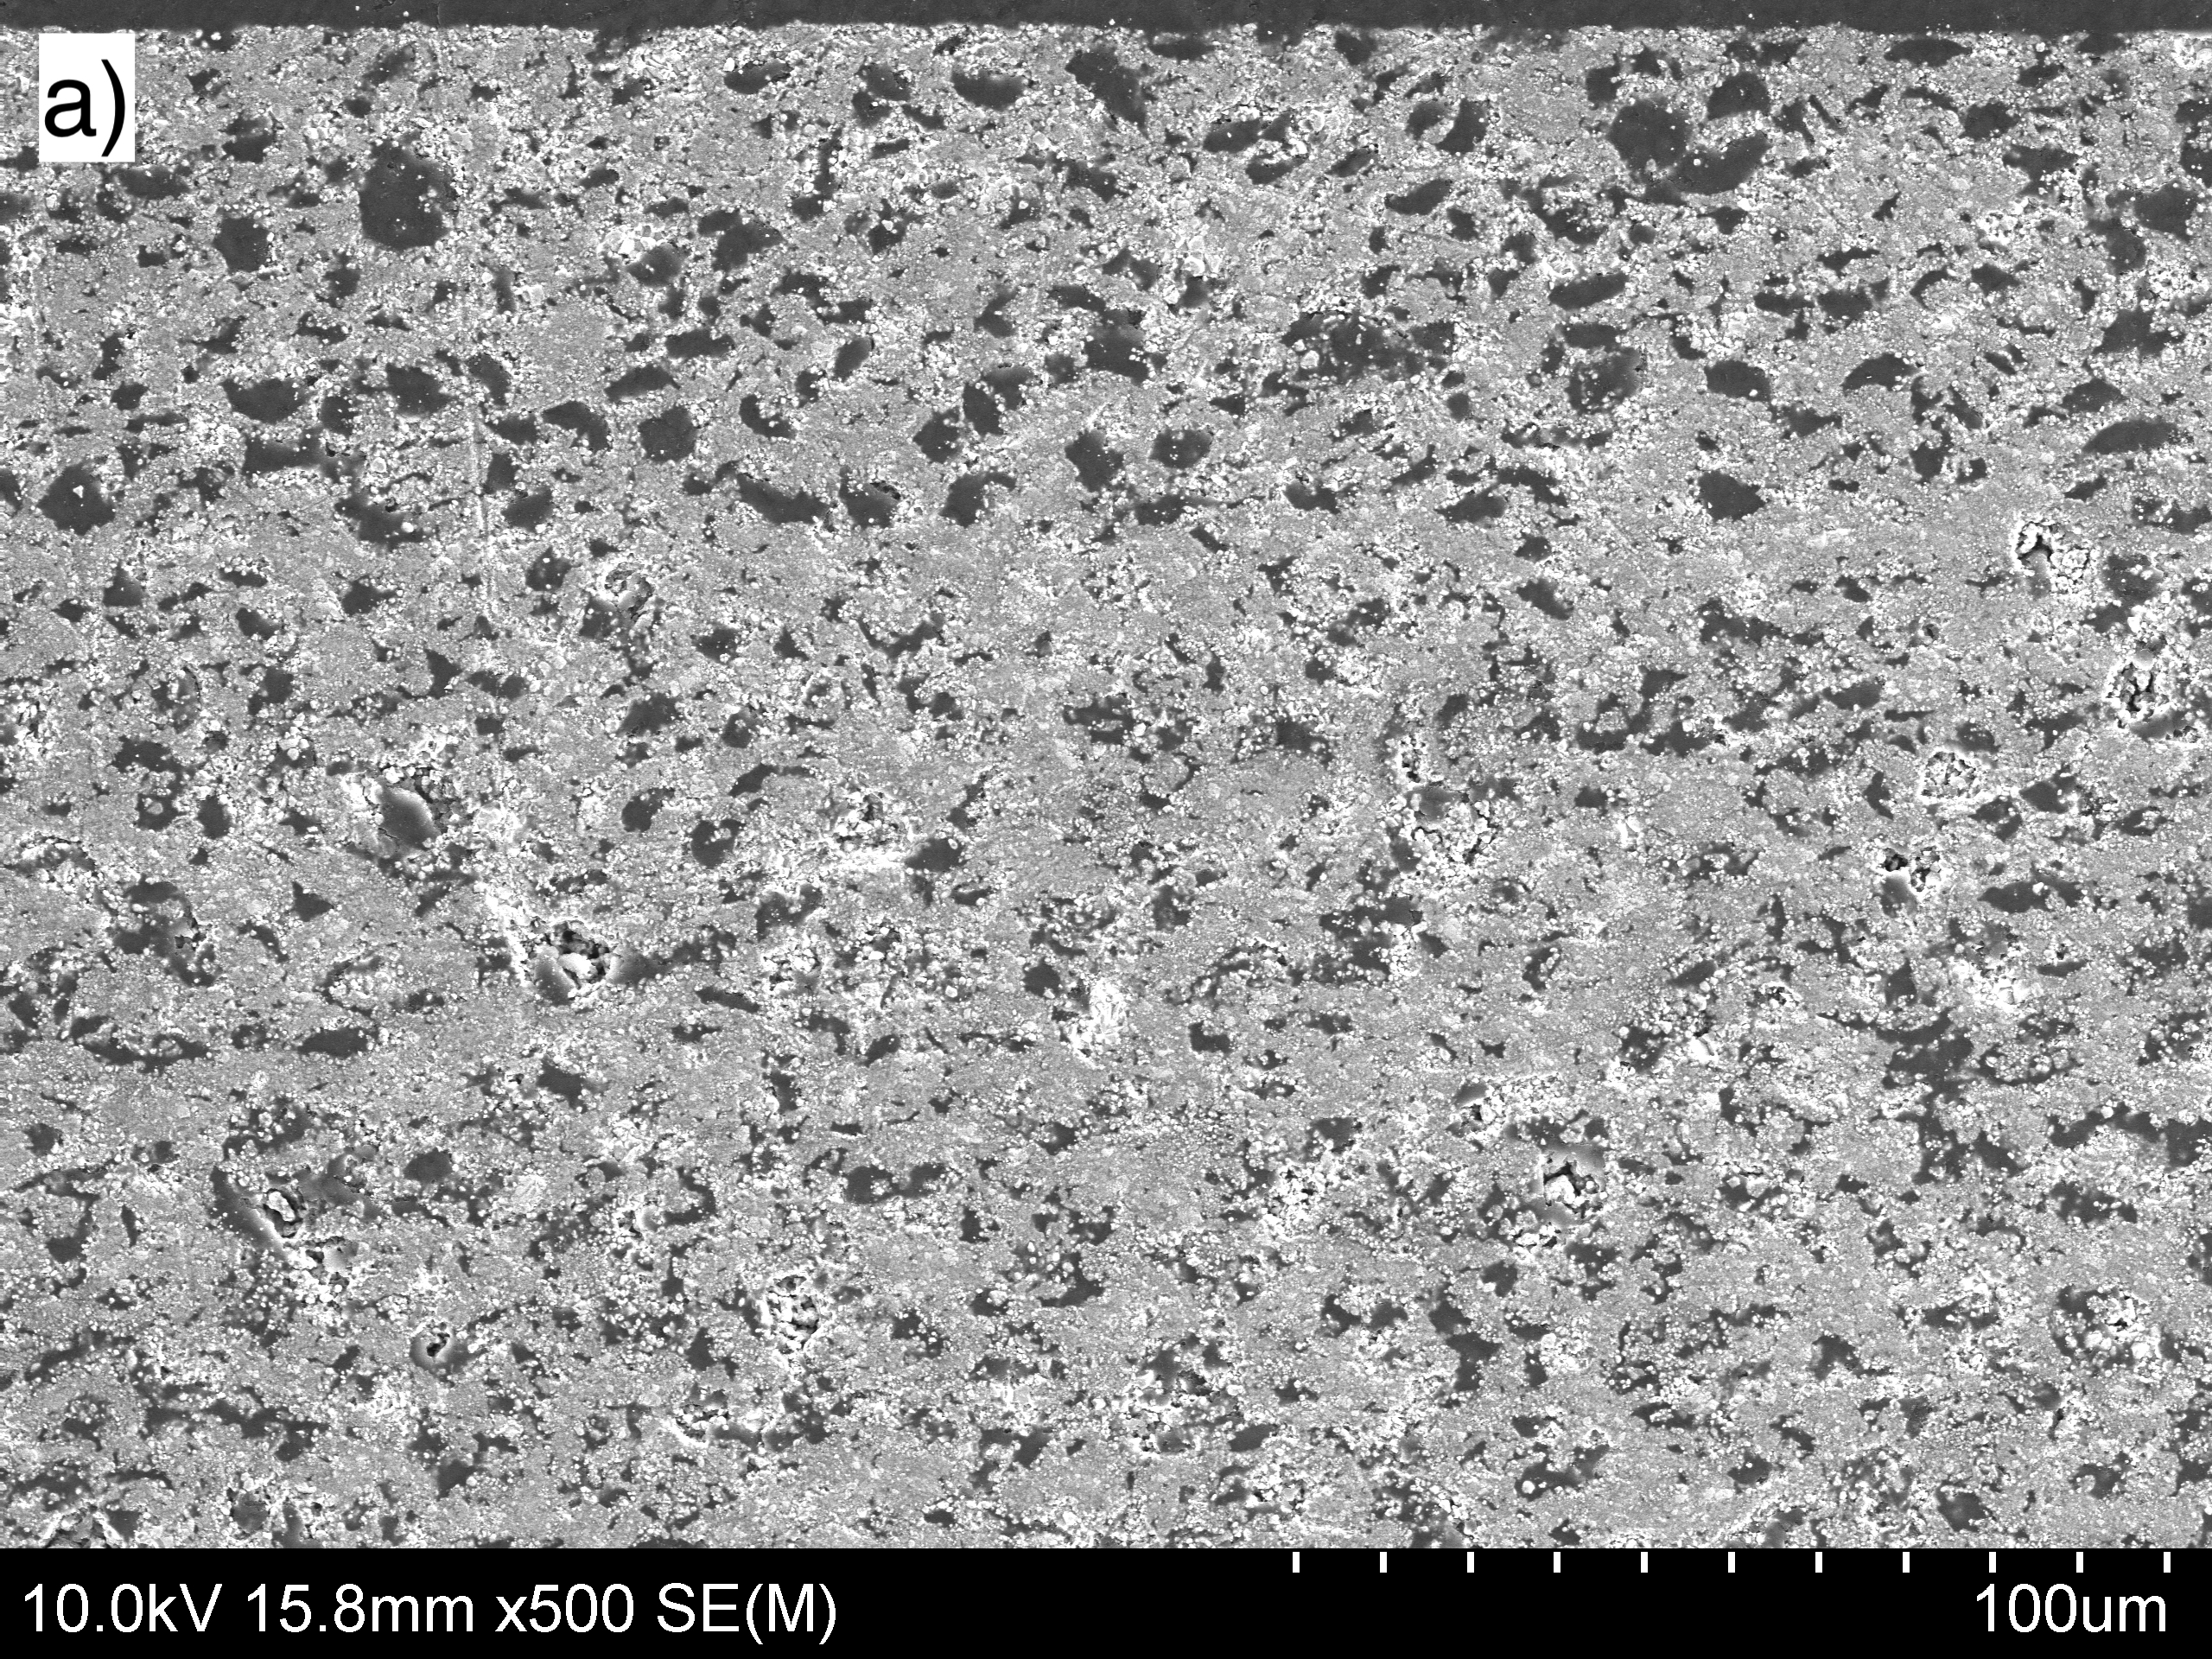
\includegraphics[width=0.45\textwidth]{0cycles.jpg}
          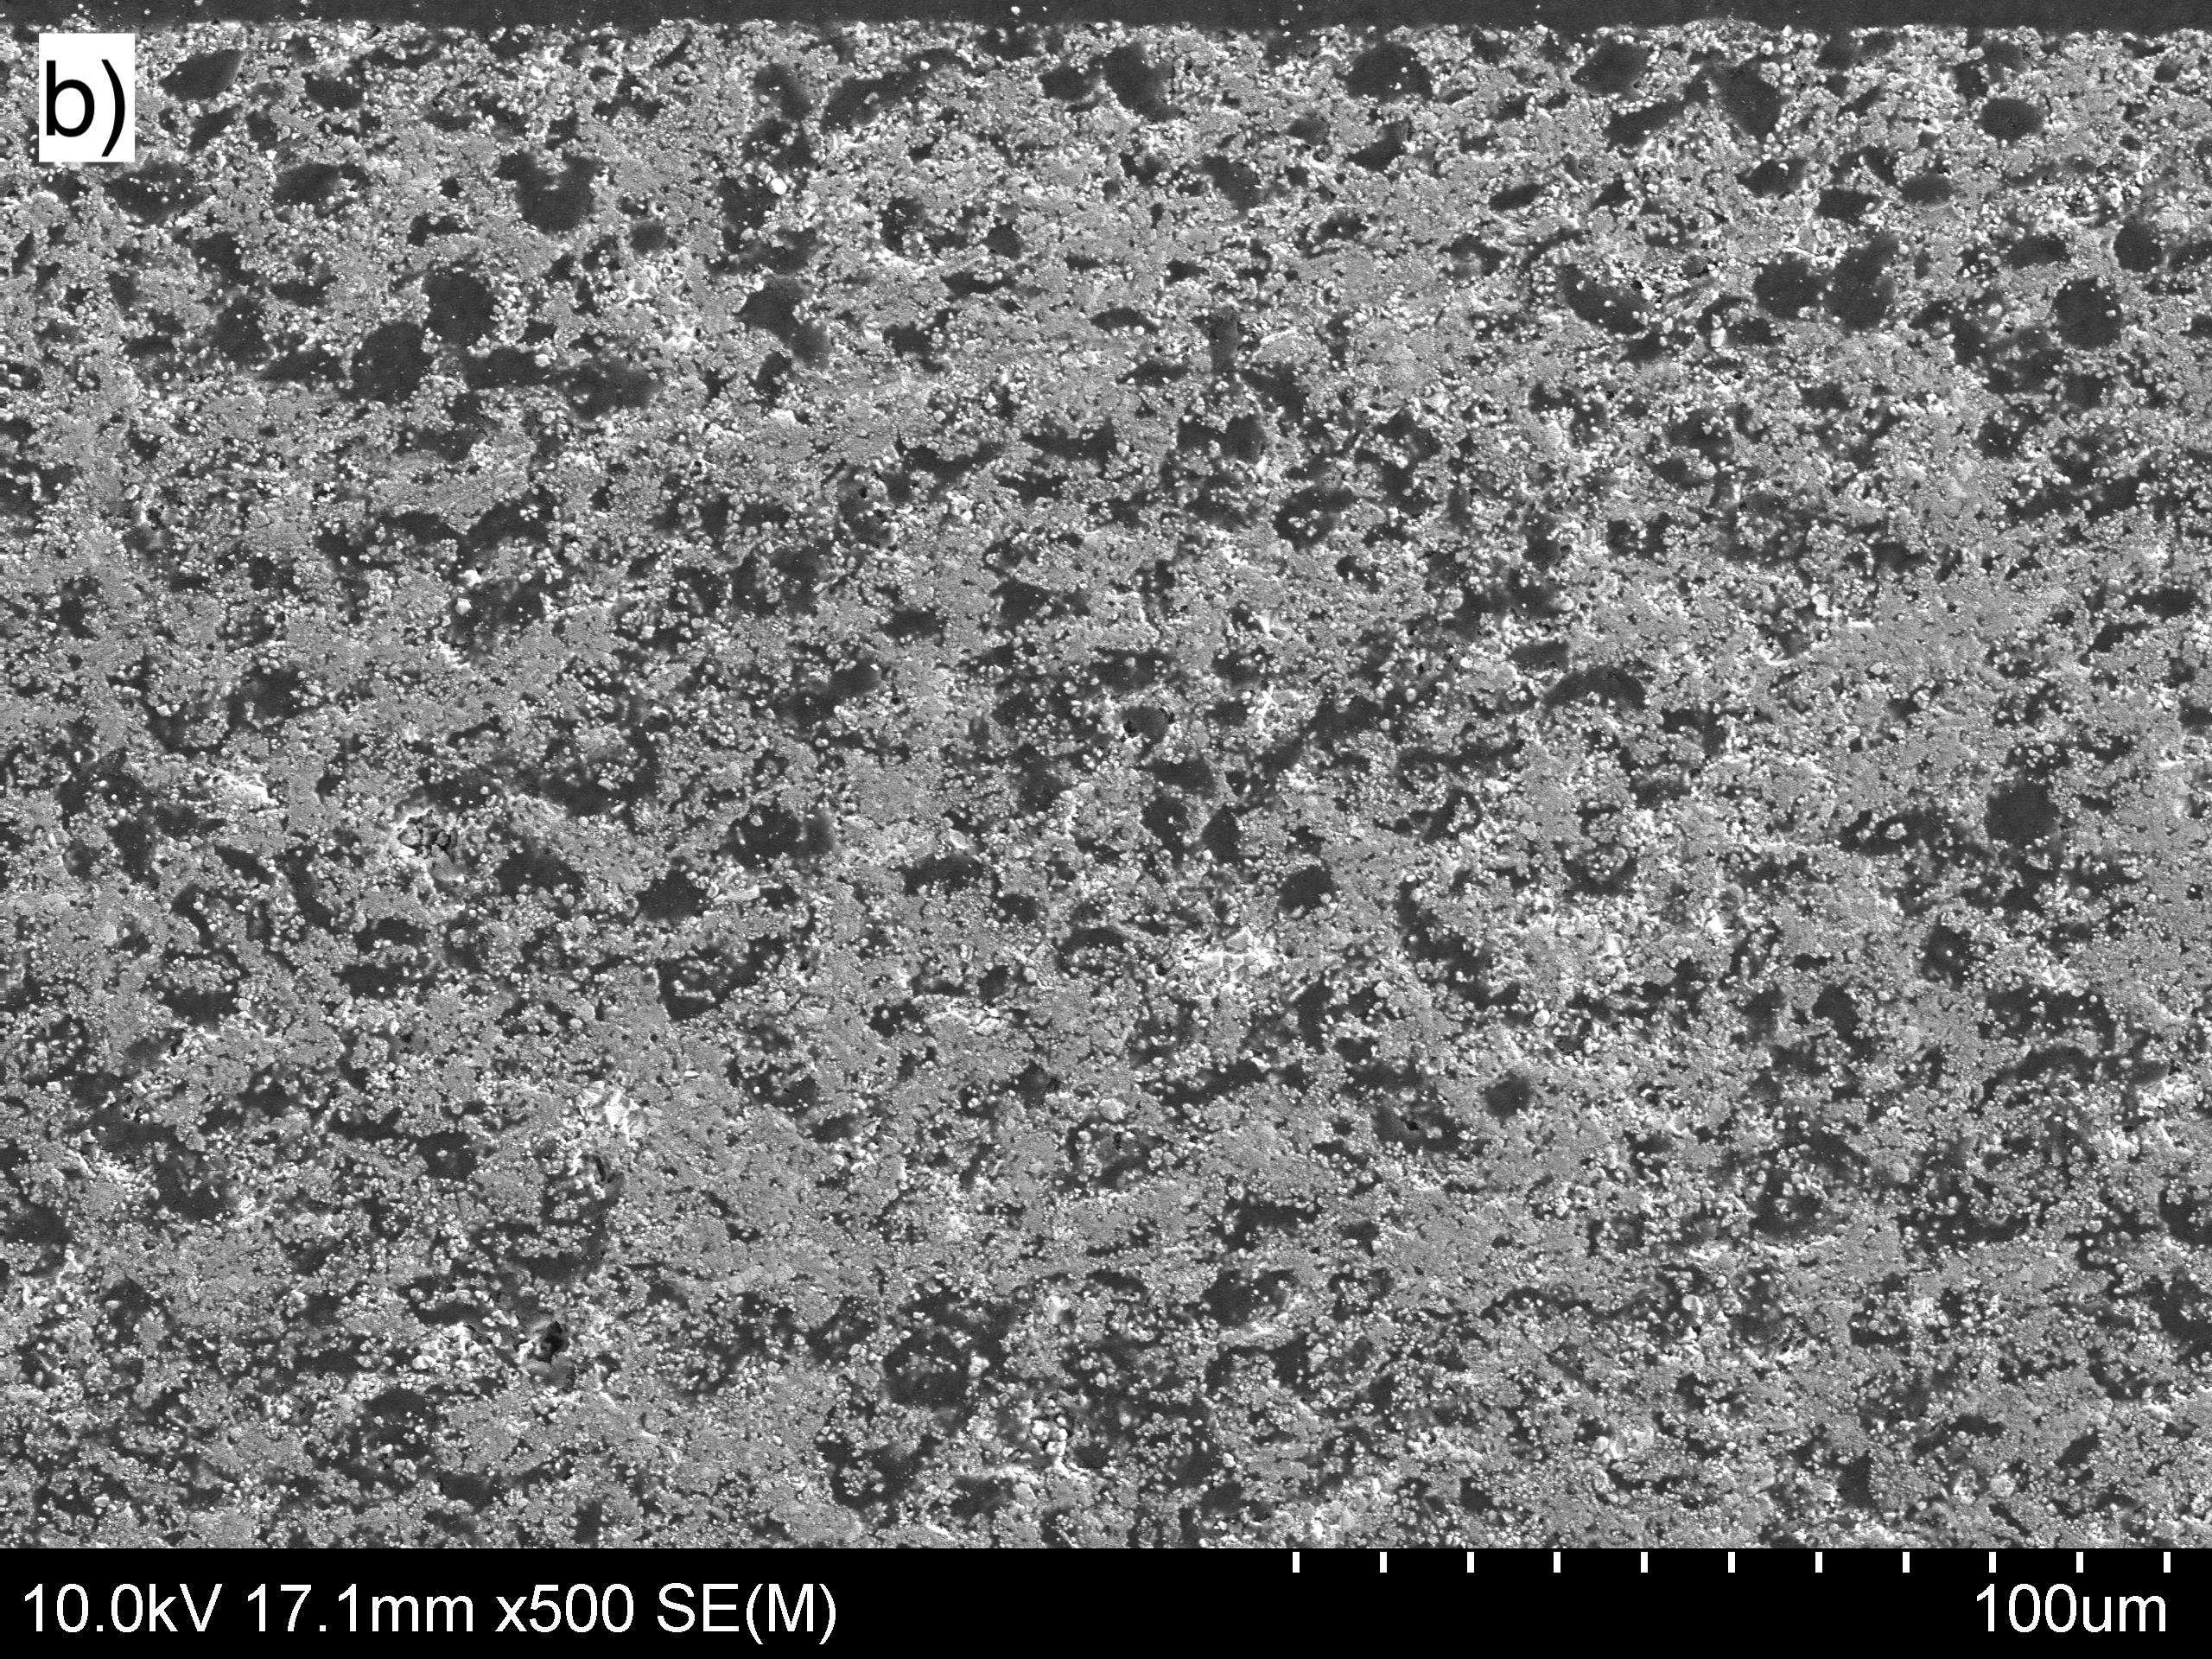
\includegraphics[width=0.45\textwidth]{10cycles.jpg}
          \caption{Scanning electron microscope images of epoxy filled and polished SFCM-GDC ASL  cross sections tested a) before any cycling, b) after 10 cycles between 10\% H\textsubscript{2} and N\textsubscript{2}.}
          \label{fig:cycledSEM}
        \end{figure}

\section{Conclusions}
    In this work the mechanical properties of SFCM and SFCM-GDC structures are characterized as the environment is changed from ambient to the working conditions of SOFCs and with redox cycling.
    The electrical conductivity of SFCM-GDC is stable up to 19 cycles due to the reversibility and phase stability of SFCM-GDC in the environment range.
    The fracture toughness of SFCM was found to be \SI[separate-uncertainty = true]{0.124 +- 0.023}{\mega\pascal\sqrt{m}} at room temperature and increases with temperature, due to relaxation of residual stresses.
    The flexural strength of SFCM-GDC/GDC half-cells increases by 23.9\% upon heating from room temperature to \SI{600}{\celsius}.
    This is due to thermal expansion pushing cracks closed during heating, requiring additional stress to propagate surface cracks and the increase in fracture toughness.
    Once exposed to reducing conditions, the flexural strength decreases by 29.4\% of the original strength, as SFCM and GDC generate oxygen vacancies.
    Reduction was shown to increase the size and variability of the distribution of flaws which lead to failure.
    Redox cycling led to the uniform increase in critical flaw size and changed the fine microstructural porosity, decreasing strength from \SI{34.3}{\mega\pascal} to \SI{22.4}{\mega\pascal}.

    These findings show that SFCM, when combined with GDC, make a suitable anode material for SOFCs.
    SFCM-GDC is a stable material system, both in terms of conductivity and mechanically, with redox cycling.
    Reduction does increase the likelihood of failure by decreasing characteristic strength and the distribution of flaws, but repeated cycling only decreases characteristic strength and does not change the Weibull modulus.

% !TEX root = ../mainthesis.tex

%Chapter 6

%\renewcommand{\thechapter}{6}

\chapter{Conclusions}

This piece will talk about \glspl{sofc}.
This is mostly because I work on \glspl{sofc}.
This is to show Mimi git.\cite{Wang2006}


\appendix
\titleformat{\chapter}
      {\normalfont\large}{Appendix \thechapter:}{1em}{}
% !TEX root = ../mainthesis.tex

%Appendix -- January 2015
%\appendix
%\renewcommand{\thechapter}{A}
%\renewcommand{\chaptername}{Appendix}

\chapter{Statistics}

\section{t-test}
    \label{app:ttest}
    The Student's t-test, or particularly the two sample t-test, is a statistical test commonly used to determine if to sets of data are significantly different from each other.
    A standard t-test creates a confidence interval around a mean for in which the true mean is thought to exist.
    By comparing the differences of two means and using the null hypothesis test to determine if the difference is zero, it can be determined if the two means are distinct, with a particular confidence.
    In the case of randomly dividing samples to receive separate treatments, this constitutes an unpaired test, as compared to a before-after sample set in which measurements are paired.
    The t-test thus gives a way to evaluating two sets of data, say flexural strength before and after reduction, and to calculate if the reduction had any significant effect.

    Like all statistical tests, this relies on a few base assumptions about the population.
    First, it is assumed that the population has a normal distribution, which reasonably fits for the samples which were studied.
    This assumption can be tested by other statistical tests, such as the Shapiro–Wilk test or Pearson's chi-squared test, or can be confirmed visually by comparing a histogram of the data to a normal distribution plot.
    The Student's t-test is not overly sensitive to the fit a normal distribution, but cases such as bimodal distributions will give inaccurate results.
    Second, for the t-test as described by Student, the two populations should have the same variance, meaning that the spread of the data compared to the mean should be equivalent, as determined by the F test.
    In the event where the variances are not equal, a variation of the t-test may be used known as the t-test for inequal variances or the Welch's t-test.
    Finally, the two populations should be sampled independently from each other.

    The t-test begins by calculating the t-score or t-value for a data set.
    The broadest and most applicable means of doing this is given by the Welch's t-test, Equation \ref{eq:studentt}, which is for sample sets with unequal variances and unequal sample sizes.
    $\overline{X}$ is the mean of the sample set, $s^2$ is the variance, and $n$ is the number of samples in the sample set.
    Because the true variance of the population is not known, the variance of the sample set is used which is the square of the standard deviation.
    \begin{equation}
        \label{eq:studentt}
        t=\frac{\overline{X}_1 - \overline{X}_2}{\sqrt{\frac{s^2_1}{n_1}+\frac{s_2^2}{n_2}}}
    \end{equation}

    Once the t-score is calculated it is compared to the critical t-score based on the confidence level desired and degrees of freedom in the measurements.
    Typically a confidence level of 95\% is used, but 99\% is also frequently found.
    This can also be referred to the level of significance, which is 1 minus the confidence level, so 0.05 or 0.01.
    In the simple case of a single set of data, the degrees of freedom is $n-1$.
    This is because for a sample set to have a given mean, all but one of the values could be any number (and thus are free), but the last value, must have a value which causes the mean to be what is expected.
    For two sample t-tests where the sets have the same number of samples the degrees of freedom become $2n-2$.
    But, for the case where the variances are unequal and measurement number may be unequal like Equation \ref{eq:studentt}, the pooled degrees of freedom must be calculated from Equation \ref{eq:dof}, known as the Welch–Satterthwaite equation.
    The degrees of freedom calculated by Equation \ref{eq:dof} is then rounded down to the next integer.
    \begin{equation}
        \label{eq:dof}
        dof=\frac{\left(\frac{s_1^2}{n_1}+\frac{s_2^2}{n_2}\right)^2}{\frac{\left(\frac{s_1^2}{n_1}\right)^2}{n_1-1}+\frac{\left(\frac{s_2^2}{n_2}\right)^2}{n_2-1}}
    \end{equation}

    With the desired confidence level and degrees of freedom calculated, the critical t-value is then looked up in a table.
    This table gives the pre-calculated t-values between which 95\% or 99\% of all values fall for the degrees of freedom in the distribution.
    If the calculated t-value is closer to zero than the critical t-value, it is determined that the two sample sets do not have a significant difference between them.
    This is because the difference between the sets falls within the range where 95\% of any random selection of two data sets from the same distribution would fall.
    Conversely, if the calculated t-value is further from zero than the critical t-value, it can be said there is a significant difference between the two and the true population means of the two sets is different.

    Many software packages will automatically calculate these values given an input dataset.
    The work in this thesis used JMP by SAS Institute to perform the calculations, but Minitab, SPSS, R, Python, Matlab, or Excel are all capable of performing the calculations with built-in functions.

\section{Weibull Statistics}
    \label{app:weibull}
    Many things in life do not have one true value, but are randomly distributed across a range of possible values, creating a distribution.
    This distribution can be modeled and analyzed to determine the likelihood of a particular outcome given the total possible number of outcomes.
    Just as there are many things which can fit a distribution, there are many different types of distributions which can represent the real world case.
    The most commonly known distribution is the normal distribution but others are frequently used and are variations on each other, such as Student's t, Lorentz, exponential, Chi-squared.
    In fracture mechanics, the Weibull distribution is used to represent the distribution of the strength of individual samples.
    The \gls{cdf} of a Weibull distribution is given in Equation \ref{eq:weibullcdf}, where $P$ is the probability of failure having occurred, $\sigma$ is the applied stress which is greater than zero, $\sigma_{min}$ is the minimum stress needed for failure, $\sigma_\theta$ is a scaling factor known as the characteristic strength, and $m$ is the Weibull modulus, or the distribution shape factor.
    Commonly there is considered no minimum stress for failure to occur, resulting in $\sigma_{min} = 0$.
    \begin{equation}
        \label{eq:weibullcdf}
        P=1-e^{-\left(\frac{\sigma - \sigma_{min}}{\sigma_\theta}\right)^m}
    \end{equation}

    The Weibull distribution was first proposed by Waloddi Weibull as an empirical fit to the observations he had been making.
    In a curious case, years later, his Weibull distribution was backed up by theory as extreme value distributions and weakest link theory was developed in the study of fracture mechanics.
    In weakest link theory, it is the result of only the largest flaw which causes failure.
    If a material has a normal, symmetric distribution of flaw sizes, then the cases of the largest flaw will be naturally skewed to the right, above the mean size and following the tail of the normal distribution.
    Of the functions which were developed for extreme values, Weibull's offered the most versatility in terms of bounds, fit and confidence intervals.

    The Weibull distribution given in Equation \ref{eq:weibullcdf} has two parameters, the characteristic strength and the Weibull modulus.
    The characteristic strength is very similar in concept to the mean of a distribution, but will always be slightly higher.
    The mean of a distribution is defined as the point where the total probability has reached 50\%.
    In contrast, the characteristic strength is defined as the point where the total probability has reached 63.2\%, or otherwise the strength which makes the exponential term of Equation \ref{eq:weibullcdf} go to $-1$.
    The Weibull modulus is a measure of the width of the distribution and thus the variability of flaw sizes and strength of the material.
    The value of the Weibull modulus depends highly on the material and the processing which occurred, but typically ranges in the 1 to 20 range.
    From an engineering perspective, a high Weibull modulus is desired because it makes the failure point more predictable.
    If multiple flaw types exist, each with their own distribution, the application of the Weibull distribution become complicated.
    Failure of each sample must be assigned the different types via fractography, and the contribution of each distribution attributed to that of the whole.

    The \gls{cdf} can be plotted linearly by rearranging Equation \ref{eq:weibullcdf} to take the form of Equation \ref{eq:weibullline}, where the slope of the line is $m$ and the intercept is $-m\ln(\sigma_\theta)$.
    This allow for fitting of the Weibull parameters and a visual estimation of if the data fits a Weibull distribution.
    The preferred fitting method is the maximum likelihood method, rather than the linear regression method, as it results in smaller confience intervals for the estimated parameters.
    \begin{equation}
        \label{eq:weibullline}
        \ln(-\ln(1-P))=m \ln(\sigma) - m\ln(\sigma_\theta)
    \end{equation}

    To achieve meaningful results with small confidence intervals, a large number of samples must be tested.
    It is best practice that for Weibull parameters to be estimated, in excess of 30 samples should be tested.
    While sometimes it is not practical to test such numbers of samples, values reported with smaller sample sets should have the confidence intervals examined.

    One unique advantage of the Weibull distribution is the ability to scale the stress applied to a sample to a different size.
    When applying stress to a relatively small sample, due to the low volume of the stressed sample, there is a low probability that a large critical flaw will be found which causes failure.
    If, one was to repeat the test on a larger sample, the added volume means a greater chance of having a critical flaw cause failure at a lower strength.
    As a result, the larger volume which is placed under stress, the weaker it will be.
    Equation \ref{eq:weibullvol} shows this relationship where $V_{E}$ is the effective volume which was placed under stress.
    For a pure tensile test, $V_E$ is the entire volume of the sample, but for flexural tests $V_E$ is much less.
    In addition to being able to scale the overall size of the sample up or down, this size scaling allows for the comparison between test methods, such as 3-point and 4-point bending.
    Using the known effective volumes from 3 and 4-point bending with similar sample dimensions and bottom spans, Equation \ref{eq:bendconvert} allows the results of the two tests to be related to each other, as long as $m$ is constant between the two test methods.
    As a result, the 3-point bend testing will always result in a greater strength compared to 4-point (as long as $m > 1$), due to the smaller volume which it engages when testing.
    \begin{equation}
        \label{eq:weibullvol}
        \frac{\sigma_1}{\sigma_2} = \left(\frac{V_{E2}}{V_{E1}}\right)^\frac{1}{m}
    \end{equation}
    \begin{equation}
        \label{eq:bendconvert}
        \sigma_{3pt} = \sigma_{4pt}\left(\frac{m+2}{2}\right)^\frac{1}{m}
    \end{equation}

% !TEX root = ../mainthesis.tex

%Appendix -- January 2015
%\appendix
%\renewcommand{\thechapter}{A}
%\renewcommand{\chaptername}{Appendix}

\chapter{TGA Manual}
\label{app:TGA}
\section{Theory of Operation}
Thermogravimetry works on the principle of measuring small changes in mass as the environment changes.
Changes in environment can come from changing temperature or gas composition.
This system uses a Cahn microbalance to measure mass, a furnace to heat the sample up to \temp{1100}, and \glspl{mfc} to control the gaseous environment.

\section{Mass Measurement}
    The TGA uses a Cahn D200 microbalance for the mass sensing capability.
    The microbalance works by measuring the current required to maintain balance between the sample and a counter balance.
    The sample can be hung at two different points on the arm of the balance, Loop A or Loop B.
    The choice of loops determines the capacity and sensitivity of the measurements, as shown in Table \ref{tab:tga}.
    Full specifications are given in the microbalance manual.
    Loop A is used most commonly for its increased sensitivity.

    \begin{table}
    \centering
    \caption{Cahn D200 Microbalance Specifications}
    \label{tab:tga}
    \begin{tabular}{lll}
                               & Loop A & Loop B                                   \\
    \cline{2-3}
    Capacity (g)               & 1.5    & 3.5                                      \\
    Maximum Weight Change (mg) & 150    & 750                                      \\
    Sensitivity (\SI{}{\micro\gram})           & 0.1    & 1                                        \\
    Repeatability              & \multicolumn{2}{l}{10\% total load on both pans}
    \end{tabular}
    \end{table}

    The microbalance has an independent flow of nitrogen gas to it to maintain a consistent atmosphere.
    Only a small amount of flow is required (\SI{5} to \SI{10}{sccm}) to keep positive pressure, but if the protective cover is removed additional time will be required to purge the balance.

    \subsection{Setup and Operation}
        Alignment of the balance is key to producing a low noise signal.
        Ideally, the hang-down wire should run through the center of the tubes and at minimum it must not touch anywhere or allow the sample pan to touch the walls of the furnace.
        The hang-down wire is made from platinum or a platinum-rhodium mixture and is in two pieces, to facilitate the changing out of the bottom portion in case of contamination and degradation.
        Two successful methods of straightening the wire are to lay it flat on a surface and roll it out from the center, similar to working dough, or to hang it with a weight and soften it using heat allowing it to stretch straight.
        Hooks on the ends are created using tweezers and a razor blade for a sharp bend.

        With the hang-down wire straight and in place, the furnace tube can be adjusted to place the sample pan in the middle, equidistance from all walls.
        Moving the tube can be achieved by adjusting the supporting clamp at the bottom of the furnace or adjusting the insulation holding it in place at the top.
        Alignment usually requires looking straight down the tube from above the microbalance.
        A light can be placed at the bottom of the tube, replacing the thermocouple, to give illumination as to the location of the sample pan in the tube.
        Alternatively, the furnace can be heated to \temp{800} so that the tube and pan glow, giving a better light, but adjustments must wait for the furnace to cool.
        Usually, both methods are used, the flashlight for a first alignment and the hot furnace to check afterwards.

        With everything aligned, the counterbalance needs to be properly adjusted.
        Place on the sample pan any appropriate crucible which will be used and open the microbalance cover and remove the cover from the counterbalance by gently pulling.
        At this point, the microbalance is turned off using the switch on the back of the microbalance controller unit.
        Counterbalance weights are added or removed to have the empty sample pan and crucible balance with the counter.
        A light touch to the arm of the balance may be needed to off-set static and friction but ensure this is done with clean tweezers.
        Once the system balances, or does so as closely as possible, the covers may be replaced and the balance turned back on.
        Static, especially in the winter time, commonly causes the counterbalance to swing wildly as the cover is placed back over it.
        Using an un-gloved hand or wiping the inside down with deionized water helps reduce the static.

        The thermocouple in the bottom of the furnace should be placed as close to the sample as possible.
        To achieve this, the thermocouple is incrementally raised while observing the mass readout from the microbalance.
        Once the balance becomes unstable or jumps, the thermocouple should be backed out \SI{0.5} to \SI{1}{\centi\meter} and tightened in place.
        The thermocouple is covered with a quartz sheath to act as a thermowell and protect the thermocouple.
        If changing between materials systems or significant degradation has occurred to the thermowell, it should be replaced.

        At this point, the system should be burned out to remove any contamination on the sample pan or hang-down wire, and time is needed for it to stabilize.
        The furnace should be heated to \temp{1000} for 4 hours in an oxygenated environment.
        This also provides time for the system to stabilize, as monitored by creating a run with the MicroScan Acquisition software.
        It can take up to 24 hours for it to stabilize.
        If random jumps occur in the mass, recheck the alignment and thermocouple placement.

        After stabilization, a sample can be loaded in to a crucible and sample pan.
        While the microbalance is calibrated to measure the mass of the sample added, it is good practice to measure and record the mass using a separate balance beforehand.
        Crucibles may be reused where appropriate.
        After the sample is placed, the furnace is raised slowly, to ensure not altering the alignment, and connected to the fittings above.
        The furnace should be at the maximum height position when finished.
        Time should then be given to allow the mass reading to stabilize before starting a test.

        The program MicroScan Acquisition controls the TGA and records data.
        After opening, select ``Balance \textgreater{} Establish Connection'' to connect to the D200.
        If an error occurs, power cycle the balance, restart the program, and check the serial cable leading to the balance.
        Upon successful connection, the current readout of the balance will be displayed.
        The balance may be tared before adding a sample by selection ``Balance \textgreater{} Tare.''
        Starting a new run is achieved by selecting ``File \textgreater{} Open Method.''
        Figure \ref{fig:tgamicroaq} shows the ``Open Method'' screen with the current balance readout from MicroScan Acquisition.

        \begin{figure}
            \begin{center}
            \includegraphics[width=0.8\textwidth,keepaspectratio]{tgamicroacq.png}
            \end{center}
            \caption{MicroScan Acquisition with Open Method open and the current read out of the balance displayed}
            \label{fig:tgamicroaq}
        \end{figure}

        From here, the total length of the run is defined along with the sample rate.
        The sample rate will need to match the rate given in the other programs.
        Additionally, the run title can be defined and the loop can be changed if needed.
        Once the run length and sample rate are entered, selecting ``Ok'' brings up the menu where the run can be started.
        Selecting ``Start Run'' causes MicroScan Acquisition to prompt for the location to save the data in a proprietary format, and once the file path is given, it then starts collecting data.
        During the run, collected data is plotted and can be viewed using the controls at the top of the plot.
        After a run is complete, the saved file is converted to a \gls{csv} by opening it with MicroScan Analysis and selecting ``File \textgreater{} Export... \textgreater{} Comma/Tab Separated...''

\section{Heating}
    Heating is done by a furnace surrounding the alumina or quartz tube and sample.
    It is controlled by a Eurotherm controller and readings are taken from a thermocouple placed inside the furnace tube.
    As a result, there is a lag in the system between the furnace elements heating and the thermocouple sensing the heat.
    The controller can be programmed with up to 8 segments in the temperature profile and programming can be performed from the front panel of the unit or by the Eurotherm iTools software.
    The iTools software must be closed before attempting to use the LabVIEW program which reads the temperature from the controller.

\section{Gas Delivery}
    Gas flows are controlled by the MKS Type 647C Multi-channel Flow Ratio/Pressure Controller and the individual MKS Type M100B \glspl{mfc}.
    Each \gls{mfc} controls one gas by measuring the flow with a thermal mass sensor and adjusting it using a valve to meet the desired set point.
    Each \gls{mfc} has a rated size and must have the zero and \gls{gfc} properly set.
    The zero can be set physically using a screw on the \gls{mfc} if a large adjustment is needed or electronically using the controller.
    The zero should be set with both sides of the \gls{mfc} open to the atmosphere to ensure no leak from a leftover pressure differential.
    The \gls{gfc} can be theoretically calculated based on the heat capacity of the gas compared to a standard.
    This assumes that the \gls{mfc} is properly calibrated, which may not be a safe assumption.
    As such, it is best to calibrate the \gls{mfc} by adjusting the \gls{gfc} so that it measures correct flow rates as given by a bubble meter.

    If an \gls{mfc} leaks despite being set to off, the tension spring for the valve located inside the \gls{mfc} may need adjustment.
    The manual for the \gls{mfc} outlines the procedure.
    If the tension is correct and the valve still leaks, service is advised.
    An alternative is to add an external shut-off valve, which can be closed either manually or automatically.
    This has been implemented for one of the current \glspl{mfc}.

    Different gases can be supplied to the \glspl{mfc} as needed for the experimental setup.
    If the gas to an \gls{mfc} is changed, a new \gls{gfc} will need to be obtained.
    Gases can humidified after the \gls{mfc} with the use of a bubbler, but they should not be humidified beforehand for risk of damaging the \gls{mfc}.
    Care should also be taken when mixing or changing gas compositions to avoid potentially dangerous combinations, such as mixing fuels and oxidizers.
    When changing between a reducing and oxidizing environment, it is good practice to allow sufficient time for a sweep gas (such as N\textsubscript{2}) to reduce the risk of the different atmospheres mixing.

    The \glspl{mfc} can be controlled by a computer with LabVIEW.
    They can either be manually set or given a scheduled program to follow.
    Typically, a constant total flow rate will be used among all tests.
    A good starting point for the total flow rate is \SI{50}{sccm}.
    After turning on the MKS controller, the master flow control must be turned on by pushing ``ON'' followed by ``0/All.''

\section{pO\textsubscript{2} Measurement}
    \po2{} of the gas flow is measured by a home-built \gls{ysz} sensor located after the \glspl{mfc} combine into one flow.
    Gas flows down a two-bore alumina tube along with a platinum wire to the end of a \gls{ysz} tube.
    The wire is lightly connected to the inside of the \gls{ysz} tube using platinum paste.
    The gas then flows in the reverse direction, between the alumina and \gls{ysz} tubes to the outlet.
    Outside the \gls{ysz} tube at the end, a separate piece of platinum wire is connected to the end of the tube.
    This setup is then placed in a furnace and heated to \temp{800} where the difference of partial pressure can be measured according to the Nernst equation.
    Voltage potentials from the two wires are measured by a Keithley 2000 digital multimeter.

    Once the system is setup, very little needs to be done to maintain the sensor.
    If the sensor needs to cooled in anticipation of a power outage or in order to be worked on, a ramp rate of \SI{1}{\celsius\per\minute} is to be used to avoid damaging the \gls{ysz} tube.
    For accurate \po2{} measurements, after any modification a calibration curve needs to be created using a reference meter.
    Voltage measurements and \po2{} calculations are recorded by the computer using a LabVIEW program.

\section{Controls}
    Almost all of the components of the \gls{tga} system are computer controllable.
    As previously mentioned and explained, the microbalance is controlled by the MicroScan Acquisition program.
    LabVIEW programs interface with the Keithley, MKS controller, and Eurotherm temperature controller.

    \subsection{Gas Controls}
        Gas flows can be controlled with either the Gas Controller or Gas Scheduler programs.
        Gas Controller allows for the immediate control of any gas flow channel while Gas Scheduler changes the gas flows at predetermined times allowing for the automated changing of composition.
        Figure \ref{fig:gascontrolfront} shows the front panel of Gas Controller, Figure \ref{fig:gasschedfront} is the front panel of Gas Scheduler, and the code for both programs is explained in Appendix \ref{app:gasvi}

        \begin{figure}
            \begin{center}
            \includegraphics[width=0.75\textwidth,keepaspectratio]{Gas_Controllerp.png}
            \end{center}
            \caption{Front panel display of Gas Controller program}
            \label{fig:gascontrolfront}
        \end{figure}

        \begin{figure}
            \begin{center}
            \includegraphics[width=0.6\textwidth,keepaspectratio]{Gas_Schedulerp.png}
            \end{center}
            \caption{Front panel display of Gas Scheduler program}
            \label{fig:gasschedfront}
        \end{figure}

        To start using Gas Controller, ensure proper channels are set for the MKS Controller Port, Arduino Port, and Servo Channel.
        On and Off position adjust the position of the external shut-off valve controlled by the Arduino.
        These values should only change if changing USB to serial adapters or with new hardware.
        Starting the LabVIEW program immediately begins the control to gasses to the specified values.
        The radio buttons on the left turn channels on or off and set them to the set point.
        To end the program, push the STOP button within the program front panel.
        The program displays the current reading for the flow to ensure flow is occurring as specified.

        The Gas Scheduler requires the input of a tab delimited text file, referred to as a schedule.
        An example schedule comes with the program.
        In this schedule, the time for the desired gas flow is given in seconds, followed by the set point of each channel.
        The program ends on the row with a negative time value, retaining those set points.

        Before starting the program, the file path to the schedule must be given by clicking the folder icon next to the Path to Program File field.
        Again, ensure that the com ports and channels are correct.
        The program records the measured flows at a set interval, as defined by the Recording Period (in seconds) and records them to a \gls{csv}.
        Additionally, comments can be added to the \gls{csv} in the optional comments field.
        After starting the program, the start button needs to be pressed.

    \subsection{Temperature and \po2{} Measurements}
        The program Temp \& pO2 Measurements reads the values from the Eurotherm controller and the Keithley multimeter, plots them, and records the results to a \gls{csv}.
        Figure \ref{fig:temppo2measure} shows the front panel of the program with the user controls.

        Before running the program, ensure that the com ports and channels are correct.
        The Measurement Period should match that given to MicroScan Acquisition.
        Enabling the timer provides for the program to stop at after the designated time.
        Comments can be added to the \gls{csv} file by filling in the File Comments field.
        When the program starts running, it will ask for the location to save the \gls{csv}.
        As a note, the timer for the program starts as soon as the program does, before defining the \gls{csv} location, but the first measurement does not occur until afterwards.

        \begin{figure}
            \begin{center}
            \includegraphics[width=0.9\textwidth,keepaspectratio]{Temp_&_pO2_Measurementsp.png}
            \end{center}
            \caption{Front panel display of Temp \& pO2 Measurements program}
            \label{fig:temppo2measure}
        \end{figure}

    \subsection{Starting a Run}
        Multiple programs needs to be started simultaneously for a run of the \gls{tga}.
        Because each program starts differently, the following is a recommendation for the order to start the programs.
        Time values from MicroScan should then be used in subsequent analysis.
        This procedure minimizes the amount of time difference between measurements on the \gls{tga}, temperature and \po2{}.

        To begin, enter all values into the various programs.
        In MicroScan Acquisition, follow the full setup, including clicking Start Run, but stop immediately afterwards with the file browser up.
        In Temp \& pO2 Measurements, follow the full setup including designating where to save the data.
        As soon as the file path to save data is submitted, switch to MicroScan Acquisition and complete the setup, submitting the file path also.
        If using Gas Scheduler, start that program as normal followed by the temperature program on the Eurotherm.

\section{Interfacing with other devices}
    The effluent of the \gls{tga} can be fed to other devices for advanced analysis, such as an \gls{ms}.
    When doing this, one thing to note is physical distance between the \gls{tga} and the other instrument.
    The longer the gas line connecting the two instruments, the longer it will take gas to travel from one instrument to the other.
    During this time period, diffusion will occur up and down the line, broadening any signal to the second instrument.
    This delay and broadening effect will need to be investigated for each experimental setup.

\section{Troubleshooting}
    \begin{itemize}
      \item \textbf{Unsteady mass:} check alignment and thermocouple placement
      \item \textbf{No gas flow on any channel:} check master flow control
      \item \textbf{No gas flow on one channel:} check if the channel is on and manual valves are open
      \item \textbf{MFC leaks when off:} Check zero, adjust spring tension as described in MFC manual, add external shutoff valve or return for repairs
      \item \textbf{No or noisy voltage from \po2{} sensor:} Check wire connections from sensor, rebuild sensor with new platinum paste
      \item \textbf{Communications Error:} Check that no other program is communicating with the hardware, restart the hardware and unplug then plug-in the USB connection
    \end{itemize}

% !TEX root = ../mainthesis.tex

%Appendix -- January 2015
%\appendix
%\renewcommand{\thechapter}{B}
%\renewcommand{\chaptername}{Appendix}

\chapter{Code}

\section{Arduino PID Relay Furnace Controller with Serial
Connectivity}\label{arduino-pid-relay-furnace-controller-with-serial-connectivity}
\label{app:PID}

The purpose of this Arduino sketch is to power a heating furnace
(controlled by a relay), with PID controls. In addition serial
communications are added to monitor, log, and interact with the
controller.

\subsection{Hardware and other
libraries}\label{hardware-and-other-libraries}

This was built to be used on a Arduino Uno R3, but should be easily run
on a variety of different boards. For temperature sensing, an
\href{https://www.adafruit.com/product/3263}{Adafruit MAX31856} is used
with the \href{https://github.com/adafruit/Adafruit_MAX31856}{library}
from them. Also used is the PID controller
\href{https://github.com/br3ttb/Arduino-PID-Library}{library by br3ttb}.
All I have really done is put the two together with the ability to
communicate over serial.

\subsection{Variables}\label{variables}

Here are a list of variables for things you may want to change based on
your setup.

\begin{itemize}
\item
  RelayPin: The physical pin your relay is connected to.
\item
  Adafruit\_MAX31856(CS, DI, DO, CLK): Pins for your MAX31856
\item
  WindowSize: Length of on/off cycle, needed to account for AC power
\item
  printdelay: Delay time in milliseconds for printout on serial
\item
  MaxOP: Maximum operating power, used to extend life of elements
\item
  myPID(\&Input, \&Output, \&workingSet,P,I,D, DIRECT): PID need to be adjusted for your setup.
  If inverse behavior is experienced (e.g. heats when it should cool) switch DIRECT.
\item
  workingSet and Setpoint: Inital setpoint for power on
\item
  ramprate: Sets a ramp rate for the working setpoint. Measured in
  milliseconds for 1C change.
\end{itemize}

\subsection{Serial communications}\label{serial-communications}

Baud rate is set to 9600. Output is tab deliminated of Setpoint, Working
Setpoint, Thermocouple Temperature, and Output Power. To change set
point, send a new number over serial and press return. You may have to
adjust your serial monitor to send \textbackslash n as end of line.

\lstinputlisting[language=C++,breaklines=true,postbreak=\mbox{\textcolor{red}{\(\hookrightarrow\)}\space}]{../../../Arduino/thermo_pid_serial/thermo_pid_serial.ino}


\renewcommand{\baselinestretch}{1}
\small\normalsize

%Assuming you are using BibTeX
\newpage
\bibliographystyle{unsrt}
\bibliography{Bibliography}

\end{document}
